%% 
%% Copyright 2007-2025 Elsevier Ltd
%% 
%% This file is part of the 'Elsarticle Bundle'.
%% ---------------------------------------------
%% 
%% It may be distributed under the conditions of the LaTeX Project Public
%% License, either version 1.3 of this license or (at your option) any
%% later version.  The latest version of this license is in
%%    http://www.latex-project.org/lppl.txt
%% and version 1.3 or later is part of all distributions of LaTeX
%% version 1999/12/01 or later.
%% 
%% The list of all files belonging to the 'Elsarticle Bundle' is
%% given in the file `manifest.txt'.
%% Template article for Elsevier's document class `elsarticle'
%% with harvard style bibliographic references
\DeclareUnicodeCharacter{03B2}{\ensuremath{\beta}}
\DeclareUnicodeCharacter{03B1}{\ensuremath{\alpha}}

%%\documentclass[preprint,12pt,authoryear]{elsarticle}

% Use the option review to obtain double line spacing
%%\documentclass[authoryear,preprint,review,12pt]{elsarticle}

%% Use the options 1p,twocolumn; 3p; 3p,twocolumn; 5p; or 5p,twocolumn
%% for a journal layout:
%%\documentclass[final,1p,times,authoryear]{elsarticle}
%%\documentclass[final,1p,times,twocolumn,authoryear]{elsarticle}
\documentclass[final,3p,times,authoryear]{elsarticle}
%% \documentclass[final,3p,times,twocolumn,authoryear]{elsarticle}
%%\documentclass[final,5p,times,authoryear]{elsarticle}
%%\documentclass[final,5p,times,twocolumn,authoryear]{elsarticle}
%% For including figures, graphicx.sty has been loaded in
%% elsarticle.cls. If you prefer to use the old commands
%% please give \usepackage{epsfig}

%% The amssymb package provides various useful mathematical symbols
\usepackage{amssymb}
%% The amsmath package provides various useful equation environments.
\usepackage{amsmath}
%% The amsthm package provides extended theorem environments
%% \usepackage{amsthm}

%% The lineno packages adds line numbers. Start line numbering with
%% \begin{linenumbers}, end it with \end{linenumbers}. Or switch it on

\usepackage{lineno}
\linenumbers
\usepackage{booktabs}
\usepackage[table,xcdraw]{xcolor}
\usepackage{lscape}

\journal{Comparative Biochemistry and Physiology Part B: Biochemistry and Molecular Biology}

\begin{document}

\begin{frontmatter}

%% Title, authors and addresses

%% use the tnoteref command within \title for footnotes;
%% use the tnotetext command for theassociated footnote;
%% use the fnref command within \author or \affiliation for footnotes;
%% use the fntext command for theassociated footnote;
%% use the corref command within \author for corresponding author footnotes;
%% use the cortext command for theassociated footnote;
%% use the ead command for the email address,
%% and the form \ead[url] for the home page:
%% \title{Title\tnoteref{label1}}
%\tnotetext[label1]{}
%\author{Coll, A.\corref{cor1}\fnref{label1}}
 %\ead{email address}
 %\ead[url]{home page}
 %\fntext[label2]{}
% \cortext[cor1]{}
% \affiliation{department={Department of Cell Biology},
%            organization={Universidad de Granada},
%            addressline={}, 
%            city={Granada},
%            postcode={}, 
%            state={},
%            country={Spain}}
% \fntext[label3]{}

%\fntext[fn1]{This is the first author footnote.}
%\fntext[fn2]{Another author footnote, this is a very long
%footnote and it should be a really long footnote. But this
%footnote is not yet sufficiently long enough to make two
%lines of footnote text.}
%\fntext[fn3]{Yet another author footnote.}
\author[1]{Alberto Coll}
\ead{albertocoll@ugr.es}

\author[2]{Amalia Pérez-Jiménez\corref{cor1}}

\author[2]{Ana E. Ortiz-Maldonado}

\author[2]{Laura Pantoja-Echevarría}

\author[3]{Marta Ramos-Barbero}

\author[3]{Eva E. Rufino-Palomares\corref{cor2}}
\ead{evaevae@ugr.es}

\author[1]{Cristina E. Trenzado}


\cortext[cor1]{Co-first author}
\cortext[cor2]{Corresponding author}



\affiliation[1]{organization={Department of Cell Biology, University of Granada},
addressline={Av. Fuentenueva, s/n},
postcode={18071},
city={Granada},
country={Spain}}

\affiliation[2]{organization={Department of Zoology, University of Granada},
addressline={Av. Fuentenueva, s/n},
postcode={18071},
city={Granada},
country={Spain}}

\affiliation[3]{organization={Department of Biochemistry and Molecular Biology I, University of Granada},
addressline={Av. Fuentenueva, s/n},
postcode={18071},
city={Granada},
country={Spain}}

\title{Assessment of stress markers in snakelocks anemone (\textit{Anemonia viridis}) in response to induced asexual reproduction} %% Article title

%% Abstract
\begin{abstract}
%% Text of abstract
\textit{Anemonia viridis} is a species of sea anemone (Cnidaria:Anthozoa) currently undergoing negative environmental impacts on their natural populations in the Mediterranean Sea. Its regeneration capacity allows for inducing asexual reproduction in captivity via longitudinal bisection, but there is no information about the impact of this procedure on the animal's physiology beyond short-term responses. The goal of this work was to assess the stress response of \textit{A. viridis} after regeneration. We measured oxidative and immunological state markers in control and bisected anemones, at 4 weeks post-injury and 20 weeks post-injury. We then performed Principal Component Analysis (PCA) to identify trends at the multivariate level. Additionally, we carried out a histological evaluation of the wound healing process during the first 7 days post-injury. Higher antioxidant enzymatic activity was found in bisected anemones, mainly in catalase and gluthathione-dependent enzymes. This response was often reverted by 20 weeks post-injury in tentacular measurements. No differences in lipid peroxidation were observed. Phosphatases activities were unaltered within the studied time-frame. Histological monitoring showed signs of amoebocyte recruitment, the immune effector cells in anthozoans, and fibrillar mesoglea organization detectable between 6 h and 24 h post-injury. Results suggest the antioxidant response could have been effective containing oxidative damage. Longitudinal fission appears to be a viable technique for inducing asexual reproduction in \textit{A. viridis} without triggering a stress response, and could reduce dependence of the market on the natural environment.

\end{abstract}

%% Keywords
\begin{keyword}
\textit{Anemonia viridis} \sep asexual reproduction \sep histology \sep innate immunity \sep oxidative stress \sep regeneration
\end{keyword}

\end{frontmatter}

%% Add \usepackage{lineno} before \begin{document} and uncomment 
%% following line to enable line numbers
%% \linenumbers

%% main text
%%

%% Use \section commands to start a section

%%\begin{linenumbers}

\section{Introduction}
\label{sec1}

The snakelocks anemone (\textit{Anemonia viridis}) (Forsskål, 1775) is a species of Cnidarian widely distributed in the Northeast Atlantic Ocean and the Mediterranean Sea. It inhabits rocky bottoms ranging from the lower intertidal zone to the subtidal, down to around 15-20 m deep, and features different colour morphs, some of which are sometimes categorized as \textit{Anemonia sulcata} (Pennant, 1777) \citep{Mallien2018, Porro2019, CalvnCalvo2020, Porcu2026}. It is also a symbiotic anthozoan that hosts photosynthetic microalgae or zooxanthellae of the genus \textit{Philozoon} (previously known as \textit{Symbiodinium} clade A temperate) \citep{LaJeunesse2022} in their gastrodermal tissue. The snakelocks anemone has been traditionally exploited for human consumption in some areas of Spain \citep{DazaCordero2002, Utrilla2019}. Illegal fishing of the species has increased in the last years and is thought to still be prevalent despite the current ban on their exploitation. Natural populations of snakelocks anemone then have to face competition with the invasive algae \textit{Rugulopteryx okamuriae}, while suffering the effects of stronger and more frequent marine heatwaves and strong exploitation pressure \citep{Suarez2020, Hamdeno2023, Pastor2023, Laamraoui2024}. 

Sea anemones are generally capable of both sexual and asexual reproduction \citep{Bocharova2016, Utrilla2019}. \textit{A. viridis} is a dioecious species featuring external fertilization, with an extended reproductive period and a spawning peak around April \citep{Utrilla2019, Porcu2026}. Vegetative asexual reproduction is widespread among sea anemones and, in the case of \textit{A. viridis}, it takes place primarily through longitudinal fission of the animal, parallel to their pharynx major axis \citep{Bocharova2016, Macias-Muoz2025}. Other mechanisms, such as budding, have been previously recorded but seem to be sporadic \citep{Utrilla2019}. Among sea anemones, vegetative asexual reproduction has been reported to occur more frequently in species and color morphs inhabiting the intertidal and shallow subtidal zones \citep{Schick1991, Mallien2018, Porro2019, Coll2025}, but it is unclear whether it is prompted by stressful environmental conditions or used to improve biological fitness by enhancing competitive ability for available space and/or maintaining optimal body size for feeding \citep{Chia1976, Sebens1979, Schick1991}. Asexual reproduction can also occur as a way of regeneration after an injury \citep{Holstein2003, Amiel2015, Bocharova2016}.

Like most cnidarians, \textit{A. viridis} is able to heal wounds rapidly and regenerate missing body parts with ease \citep{Parisi2020, LaCorte2023}. Artificial sectioning of this species can trigger regeneration of the missing body parts yielding two clonal anemones, but it is also an invasive process than can induce stress in the animals. Generation of reactive oxygen species (ROS) is known to occur during wound healing and regeneration in sea anemones and other anthozoans, due to metabolic activation, though the temporal scope of this response is still unclear   \citep{Mydlarz2006, Parisi2020, LaCorte2023, Vullein2024, Mack2025}. ROS are generated as a by-product of oxidative phosphorylation, and can act as signaling elements of apoptosis, proliferation and differentiation pathways that are crucial to regeneration \citep{Gauron2013, Vullein2024, Mack2025, Vullien2025}.  However, while ROS perform important roles during these processes, imbalances between ROS generation and scavenging can result in damage to cellular lipids, proteins or DNA. Uncontrolled ROS production can potentially impact short-term health of the organism during these physiological processes and may persist after the regeneration process is over \citep{Lesser2006, Lushchak2011}.

Hence, ROS production must be counterbalanced with different antioxidant defence mechanisms, which may be enzymatic or non-enzymatic (also known as low-molecular-weight) in nature \citep{Lesser2006}.  Superoxide dismutase (SOD) scavenges superoxide anion and converts it into $\mathrm{O_2}$  and $\mathrm{H_2O_2}$, acting as a first line of defense against ROS. Because $\mathrm{H_2O_2}$ is not charged, it can diffuse across biological membranes and cause oxidative damage not restricted to the generation site \citep{Lesser2006}. $\mathrm{H_2O_2}$ scavenging is crucial to avoid generation of the more reactive hydroxyl radical, and both catalase (CAT) and glutathione peroxidase (GPx) fulfill this role in different cellular compartments \citep{Lesser2006, Lushchak2011}. GPx, however, is dependent on the availability of reduced glutathione, a low molecular-weight antioxidant which is regenerated by the activity of glutathione reductase (GR) \citep{Couto2016}. While not part of the main ROS-scavenging systems, glutathione S-transferases (GST) are a family of Phase II detoxifying enzymes that are able to conjugate glutathione to different xenobiotics, as well as scavenging ROS \citep{Couto2016}. NAD(P)H:quinone oxidoreductase 1 (NQO1) is an enzyme that reduces quinonoid compounds generated by the electron transport chain, preventing semiquinone formation and ROS production \citep{Atia2020, Ross2021}.

However, changes in antioxidants markers cannot be interpreted on their own in the context of oxidative balance. It is also necessary to study oxidative damage markers to assess both the responses that organisms develop in order to face stressors and the adverse effects that they experience when doing so \citep{Beaulieu2014}. For instance, increases in antioxidant enzymes activity coupled with higher oxidative damage might indicate that there was mobilization of antioxidant defenses, but it was unable to fully protect against oxidative damage \citep{Beaulieu2014}. One of the most used marker of oxidative damage is malondialdehyde, an end-product of lipid peroxidation that can be assayed quickly and inexpensively through the thiobarbituric acid reactive substances (TBARS) assay \citep{AguilarDiaz2020, Buege1978}.

Biomarkers of oxidative stress are advantageous because they are not confined to a certain taxonomic range: they can be assessed in any organism that has aerobic metabolism or is exposed to oxygen. The universality of these markers makes them highly valuable when studying basal invertebrate phyla, where other key stress markers in vertebrates, such as glucocorticoids, have been seldom studied \citep{Beaulieu2014, Coll2025, Valavanidis2006}. In the particular case of cnidarians, some studies have detected the presence of steroid hormones, including hydrocortisone, in different Hydrozoans and Anthozoans \citep{Nikitina2024}. However, no steroid receptor coding genes have been found in the phylum, and regulatory pathways of steroid compounds remain largely unstudied \citep{Tarrant2007, Baker2015}. 

Cnidarian immunity is fundamentally innate and is comprised of processes of pattern recognition, intracellular signaling, followed by effector responses, and tissue repair \citep{Parisi2020}. Regarding cellular responses, mass recruitment and proliferation of amoebocytes, the immune effector cells in anthozoans, has been described both in \textit{A. viridis} and other hexacoral anthozoans during wound healing \citep{Vargas-Angel2007, Mydlarz2008, Parisi2020, Snyder2021, LaCorte2023}. Anthozoans feature granular and hyaline amoebocytes, sometimes referred to as granulocytes and hyalinocytes, respectively \citep{Fabrello2023}. These cells are motile through the mesoglea, exhibit phagocytic activity, are involved in transport of glycogen, and, in some cnidarian species, have been reported to exhibit respiratory burst as an immune mechanism \citep{Larkman1984, Mydlarz2004, Mydlarz2006, Parisi2014, Snyder2021, Fabrello2023, LaCorte2023}. Other effector responses of the cnidarian immune system involve activation of different hydrolases such as acid and alkaline phosphatase, which are known regeneration markers in this taxon \citep{Trapani2016, Konada2020, Parisi2020}.

In the present study, we studied the physiological responses of the snakelocks anemones (\textit{Anemonia viridis}) after induction of asexual reproduction to generate two clonal individuals. We studied whether this process affects the stress response of the snakelocks anemone, through evaluation of biochemical markers of oxidative and immune status, and through histological evaluation of morphological changes after the regeneration process. Because of the intrinsic correlation that physiological markers exhibit, we used Principal Component Analysis to examine the correlational structure of these markers and identify driving variables of the dataset at a multivariate level.


\section{Materials and Methods}
\label{sec2}

\subsection{Experimental design and sampling}
\label{subsec1}

In November 2020, 300 wild anemones were obtained from natural environments off the coast of Granada (Spain) with the corresponding permits from local authorities. To ensure representation of different populations of the area, three sampling points were selected in Calahonda (36º42’11.0”N, 03º24’45.5”W), Salobreña (36º44’12.2”N, 03º35’35.1”W), and Almuñécar (36º 44’41.8”N, 03º39’41.9”W). Animals were transferred to facilities of Andalmar Biotech S.L., where they were kept in a concrete 16 m$^3$ outdoor tank, set under a 0.5 mm white nylon mesh cover. 

Anemones from the three sampling points were pooled and distributed in 11.8 L floating baskets at a density of 16-17 individuals per basket, making a total of 18 baskets. An Integrated Multitrophic Aquaculture (IMTA) culture environment was established to mimic the natural environment, where other organisms were co-cultured in the same system as per previous studies \citep{Coll2025}. The composition of the IMTA environment was the following: beadlet anemones (\textit{Actinia equina}), sea urchins (\textit{Paracentrotus lividus}, \textit{Arbacia lixula}), sea snails (\textit{Monodonta turbinata}), limpets (\textit{Patella caerulela}), sea cucumbers (\textit{Holothuria tubulosa}), mussels (\textit{Mytillus edulis}), and two macroalgae species (\textit{Ulva rigida}, \textit{Cystoseira mediterranea}).

The tank was equipped with a recirculation system consisting of a mechanic sand filter, biological filter with 300 m$^2$/m$^3$ bio-balls and protein skimmer. Natural seawater was pumped from a well in the facilities and then filtered to be used in the circuit. Salinity and pH were monitored during the experimental period, centered around 34.8 ‰ and pH 8. Natural photoperiod was used, and water temperature varied with ambient temperature, with an overall mean of 17.5º C (minimum of 9º C - maximum of 27º C) throughout the study.

After acclimation to the aquaculture conditions for one month, nine baskets were selected as the experimental group, and anemones in them were sectioned in half through their pharynx major axis. Each of the resulting halves was returned to their original baskets and left to heal, in order to generate two different clonal individuals. The remaining baskets and anemones were labeled as controls. In order to control for the handling that bisected anemones suffered and to ensure clonal anemones are identified, all specimens were placed on mortar disks within the floating baskets. Adhesion to these mortar disks also facilitated handling of the animals during the rest of the experimental period.

The first sampling (T1) took place four weeks post-injury, once the anemones had had time to heal completely. Eighteen anemones of similar size (approximately 30 mm of oral disk diameter) and phenotype (\textit{vulgaris} colour morph, as described by \citet{Porro2019} were randomly selected from the control and bisected baskets, making a total of 9 control anemones and 9 bisected anemones (one per basket). A second sampling (T2) took place 20 weeks post-injury, following the exact same procedure and thus resulting in a total sample size of 36 individuals. 

At both sampling events, each anemone was snap-frozen in liquid nitrogen and stored at -80º C. Due to tentacles containing greater zooxanthellae density and being sites of ROS production associated with photosynthesis, they were dissected and processed separately from the column. Samples were homogenized (Heidolph Instruments) in 100 mM Tris, 0.1 EDTA and 0.1\% Triton buffer (pH 7.8) at a 1:4 ratio (w/v). Extracts were then centrifuged at 16,000 rpm for 30 minutes at 4º C (Sigma 3 K30), and the supernatant was collected, distributed in aliquots and stored at -80º C for subsequent analysis. 

Additionally, mortality was recorded within the control and bisected group during the experimental period. The remaining anemones were left to heal and grow, and in June 2020, were released into the natural environment as part of project ORTIMAR (FB2019-1). 

\subsection{Oxidative status assays}
\label{subsec2}

All oxidative parameters measurements were carried out with a PowerWave microplate spectrophotometer (Bio-Tek Instrument, Inc.) at a stable temperature of 25 °C for enzymatic determinations. Technical replicates were used for all determinations. Superoxide dismutase (SOD) (EC 1.15.1.1) activity was determined according to \citet{McCord1969} method, consisting of an indirect measurement as the degree of inhibition of cytochrome c reduction. Determination of catalase (CAT) (EC 1.11.1.6) activity was performed using \citet{Aebi1984} method, based on the decrease in absorbance produced by $\mathrm{H_2O_2}$ consumption by this enzyme.

Glutathione peroxidase (GPx) (EC 1.11.1.9) activity of the samples was determined following \citet{Floh1984} method, based on an indirect measurement of NADPH oxidation, generated by its coupling with a standard glutathione reductase (GR) (EC 1.8.1.7) reaction. GR activity was measured according to \citet{Carlberg1975} method, consisting on a measure of the absorbance decrement caused by NADPH oxidation. Glucose 6-phosphate dehydrogenase (G6PDH) (EC 1.1.1.49) activity of the samples was obtained using a modified method of \citet{Lhr1965}, based on recording the change in absorbance due to NADPH production by the enzyme.

Determination of glutathione S-transferase (GST) (EC 2.5.1.18) activity was performed following the method of \citet{Frasco2002}, based on the formation of a conjugate between glutathione and 2,4- dinitrochlorobenzene that increases absorbance. NAD(P)H:quinone oxidoreductase 1 (NQO1, also known as DTD) (EC 1.6.99.2) activity was determined using a modified method of \citet{Lemaire1996}, based on measurement of the decrease in absorbance caused by reduction of 2,6-dichlorophenol indophenol.

Soluble protein content was quantified following \citet{Bradford1976} method in order to express enzymatic specific activity. One unit of activity was defined as the amount of enzyme required to transform one $\mathrm{\mu}$mol of substrate per minute under the measurement conditions. For SOD, units of activity were defined as the amount of enzyme required to generate a 50\% inhibition in the reduction of cytochrome c.

Total antioxidant activity was measured according to \citet{Erel2004} method, based on the change of absorbance due to reduction of 2,2'-azino-bis-(3-ethylbenzothiazoline-6-sulfonic acid), to determine Trolox-equivalent antioxidant capacity (TEAC) of the extracts. Last, oxidative damage to lipids was assayed as thiobarbituric acid reactive substances (TBARS) content, following a modified method from \citet{Buege1978} and using malondialdehyde (MDA) as a standard. 


\subsection{Immune status parameters}
\label{subsec3}

Immune parameters measurements were performed in technical replicates, using a PowerWave microplate spectrophotometer (Bio-Tek Instrument, Inc.) at a stable temperature of 25 °C. Acid (EC 3.1.3.2) and alkaline (EC 3.1.3.1) phosphatase (ACP and ALP respectively) activities were measured following the method of \citet{Huang2011}, based on the change of absorbance produced by the activity of the enzyme on p-nitrophenyl at pH 5.0 and 8.0, respectively. Solution pH was adjusted through addition of HCl or NaOH. Determination of myeloperoxidase (MPO) activity (EC 1.11.1.7), an enzyme involved in respiratory burst in macrophages, was carried out following a modified method of \citet{Mohanty2010}, based on the increase of absorbance due to oxidation of 3,3',5,5'-tetramethylbenzidine (TMB) by the products of MPO activity. One unit of activity was defined as the amount of enzyme required to transform one $\mathrm{\mu}$mol of substrate per minute under the measurement conditions.  

\subsection{Histology}
\label{subsec4}

For histological characterization, a different subset of twelve individual anemones were subjected to the bisection procedure. Animals were kept in 3 polyester fiber 500 L tanks, with a common filtration tank, provided with mechanical filtration media (industrial foam) and 10 L of bio-balls (Kaldnes). Recirculation was established using a pump (Sicce Multi, 2500 L/h 50W). Natural illumination was complemented with 15W-6400K white LED lights programmed to match natural photoperiod. Temperature oscillated with ambient temperature, with a mean of 25º C during the experiment (minimum of 20º C - maximum of 28º C).

Samples were taken immediately, 6 hours, 24 hours and 7 days  after the injury, using 3 replicates per time point. All anemones displayed the \textit{vulgaris} colour morph \citep{Porro2019} and had similar sizes (approximately 30 mm of oral disk diameter) to reduce possible sources of variability in regeneration time. From one of the two halves of the bisected anemones, a small portion which included the original injury was dissected and fixed in 4\% PFA for 24 h. After histological processing, paraffin-embedded tissue blocks were sectioned at 5 micrometers using a rotary microtome (Leica RM 2135). Histological sections were deparaffinised and stained with Masson-Goldner trichrome stain (Sigma-Aldrich) for light microscopy observation (Leica DM2000 and coupled Leica ICC50 W camera) and descriptive analysis of the injured body wall.

\subsection{Statistical analysis}
\label{subsec5}

All statistical analysis and data processing was carried out using R. 4.4.3 and Rstudio 2024.12.1. Results were expressed as arithmetic mean ± standard error of the mean (SEM). A confidence level of 95\% ($\alpha$ = 0.05) was established for all statistical tests. A Chi-square test of Independence was performed to test for association between mortality rate and experimental group. For each biochemical marker, a two-way ANOVA (Type II) was conducted to examine the effect of the reproduction procedure (treatment) at short and time on the stress response of \textit{A. viridis}. Assumptions of normality of residuals and homoscedasticity were assessed via Shapiro-Wilk’s normality test and Levene’s test. All residuals were normally distributed (p > 0.05) and all variables had homogeneity of variances (p > 0.05). When interaction between both variables was found to be significant, differences between groups were assessed visually by calculating the estimated marginal means for each group with a 95\% confidence interval (CI), as proposed by \citep{Garofalo2022}. Groups with little to no overlap (< 25\%) were considered to have different estimated marginal means.

Additionally, principal component analysis (PCA) was performed separately on columnar and tentacular variables to examine correlational structure of the data and identify main drivers of the differences between control and bisected anemones. Mardia's test was used to check multivariate normality, and Barlett's test of sphericity was used to check distinction from the identity matrix. Significance of the PCA, loadings and principal components was assessed via permutation tests on the  $\psi$ and $\phi$ statistics proposed by \citet{Vieira2012}, using the R package PCAtest \citep{Camargo2022}.

\section{Results}
\label{sec3}

\subsection{Mortality rate}
\label{subsec6}
No mortality was recorded within the control baskets throughout the experimental period. The bisection procedure registered a 7.9\% overall mortality (data not shown). The relation between mortality rate and experimental group was significant ($\chi^2_{(1, N=300)}$ = 10.352, p = 0.001, $\phi=0.186$).

\subsection{Oxidative status assays}
\label{subsec7}
Complete results of the two-way ANOVA are gathered in detail in Supplementary Table 1. SOD activity (Figure \ref{fig:sod}.A) featured no significant effects of treatment, time or interaction between them on columnar samples. Tentacular SOD activity similarly featured no significant effects of treatment, time or interaction. Columnar CAT activity (Figure \ref{fig:sod}.B) was higher in bisected anemones ($F_{(1,32)}$= 8.89, p = 0.027), but there was no effect of time or interaction. Tentacular CAT activity did not show significant effects of either treatment or time, but it featured significant interaction between them ($F_{(1,32)}$= 27.85, p = 0.001). Visual examination of the estimated marginal means and their 95\% confidence intervals (Figure \ref{fig:emm1}.A) showed that bisected anemones had a higher mean CAT activity than control ones at T1, but this tendency was inverted at T2.

\begin{figure}[htb]
    \centering
    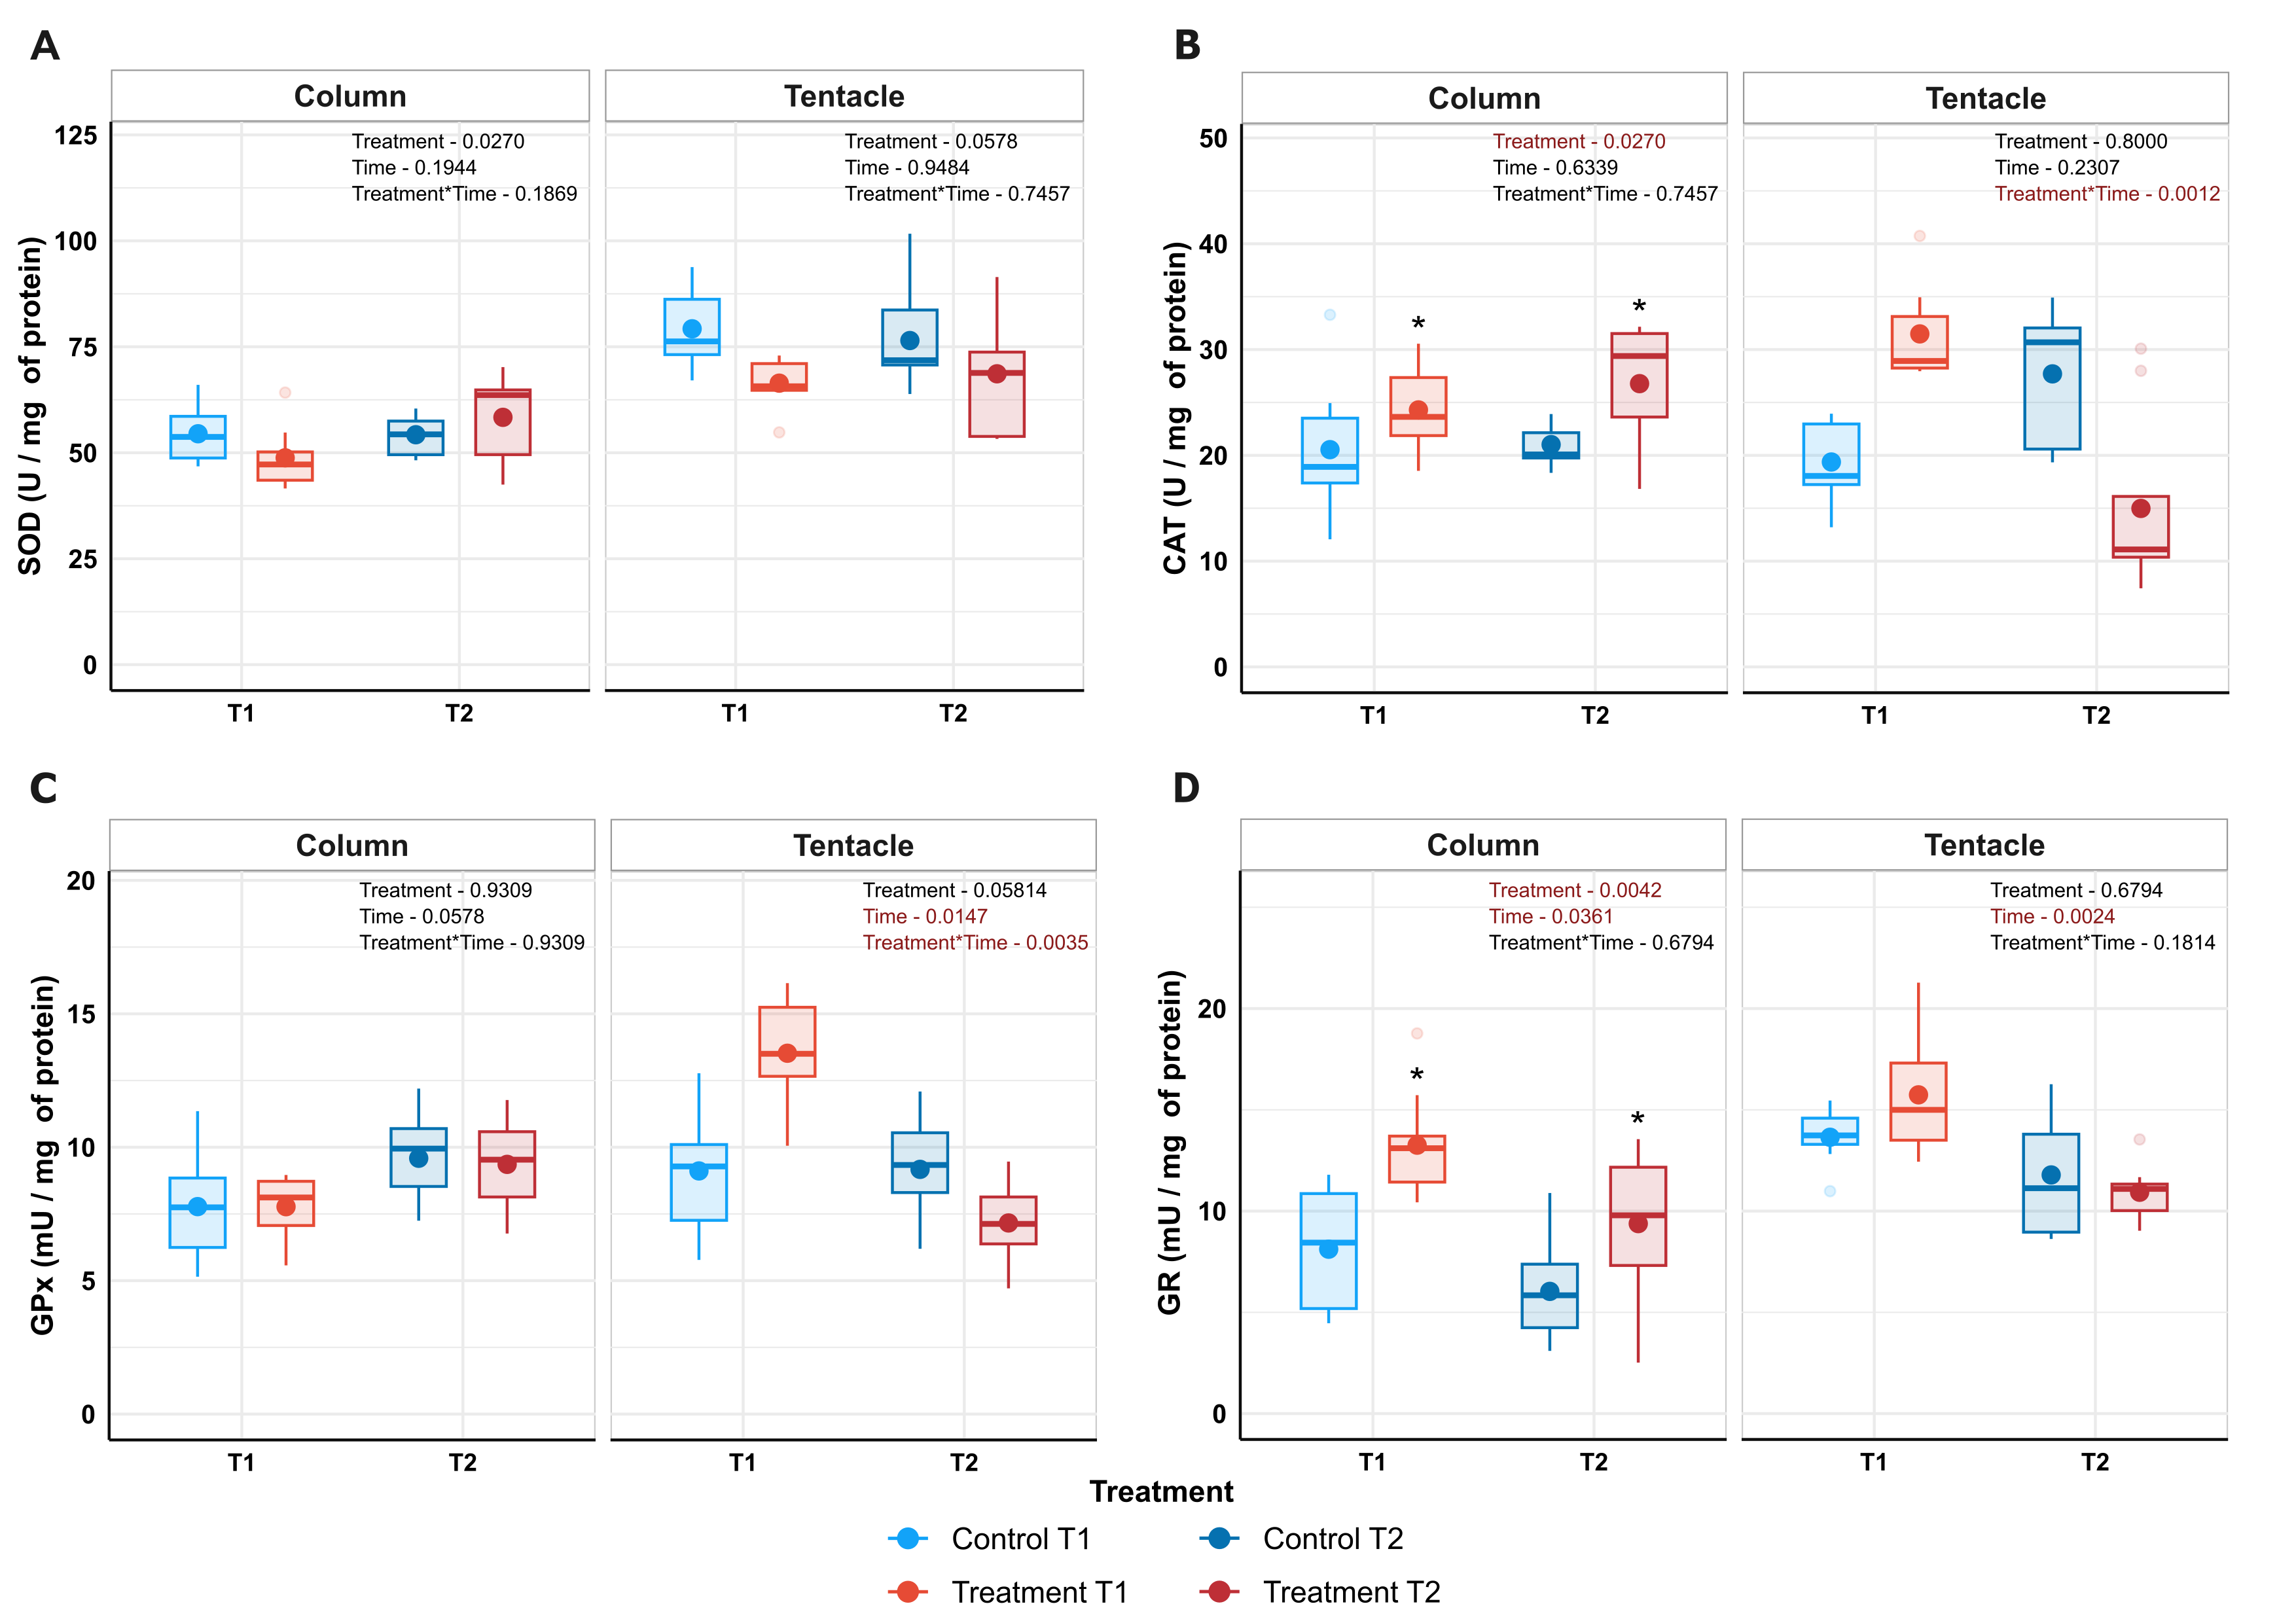
\includegraphics[width=1\textwidth]{fig_boxplot1.png}
    \caption{(A) Superoxide dismutase (SOD), (B) catalase (CAT), (C) glutathione-peroxidase (GPx) and (D) glutathione reductase (GR) activity on column and tentacles of control and bisected anemones, at T1 (4 weeks) and T2 (20 weeks). Coloured dots represent the mean activity. n = 9 per experimental group. Two-way ANOVA table is displayed on each panel, with p-values < 0.05 in red. Asterisks indicate significant differences due to treatment main effect. Effects of time not indicated.}
    \label{fig:sod}
\end{figure}

Columnar GPx activity (Figure \ref{fig:sod}.C) was not affected by treatment, time or their interaction. Similarly, there was no significant effect of treatment on tentacular GPx activity, but it was affected by time ($F_{(1,32)}$= 11.54, p = 0.015) and treatment by time interaction ($F_{(1,32)}$= 17.68, p = 0.003). Visual examination of estimated marginal means (Figure \ref{fig:emm1}.B) showed that, at T1, bisected anemones had a higher mean GPx activity than control anemones. This difference was non-existent at T2, where activity levels are similar between control and bisected anemones. Regarding GR activity, bisected anemones featured higher columnar activity (Figure \ref{fig:sod}.D) than control anemones regardless of time ($F_{(1,32)}$= 16.28, p = 0.004), and activity was found to be lower at T2 than T1 ($F_{(1,32)}$= 8.06, p = 0.036), but there was no significant interaction between both variables. Tentacular GR activity was also lower at T2 ($F_{(1,32)}$= 20.11, p = 0.002), but there was no effect of treatment or treatment by time interaction on this variable.

There was no effect of treatment, time or their interaction on columnar GST activity (Figure \ref{fig:gst}.A). However, tentacular GST activity was significantly affected by time ($F_{(1,32)}$= 23.91, p = 0.0008) and interaction ($F_{(1,32)}$= 17.58, p = 0.004). Visual examination of estimated marginal means (Figure \ref{fig:emm2}.A) revealed that bisected anemones at T1 had higher mean activity than controls at T1, but also than both T2 groups. Columnar NQO1 activity (Figure \ref{fig:gst}.B) increased significantly on bisected anemones ($F_{(1,32)}$= 11.21, p = 0.015), but there was no effect of time or interaction. However, there was a significant effect of treatment ($F_{(1,32)}$= 19.34, p = 0.003), time ($F_{(1,32)}$= 10.87, p = 0.020) and treatment by time interaction ($F_{(1,32)}$= 8.96, p = 0.027) on tentacular NQO1 activity. Visual examination of estimated marginal means (Figure \ref{fig:emm2}.B) showed that, once again, bisected anemones at T1 had higher mean activity than controls at T1 and both T2 groups.

\begin{figure}[ht]
    \centering
    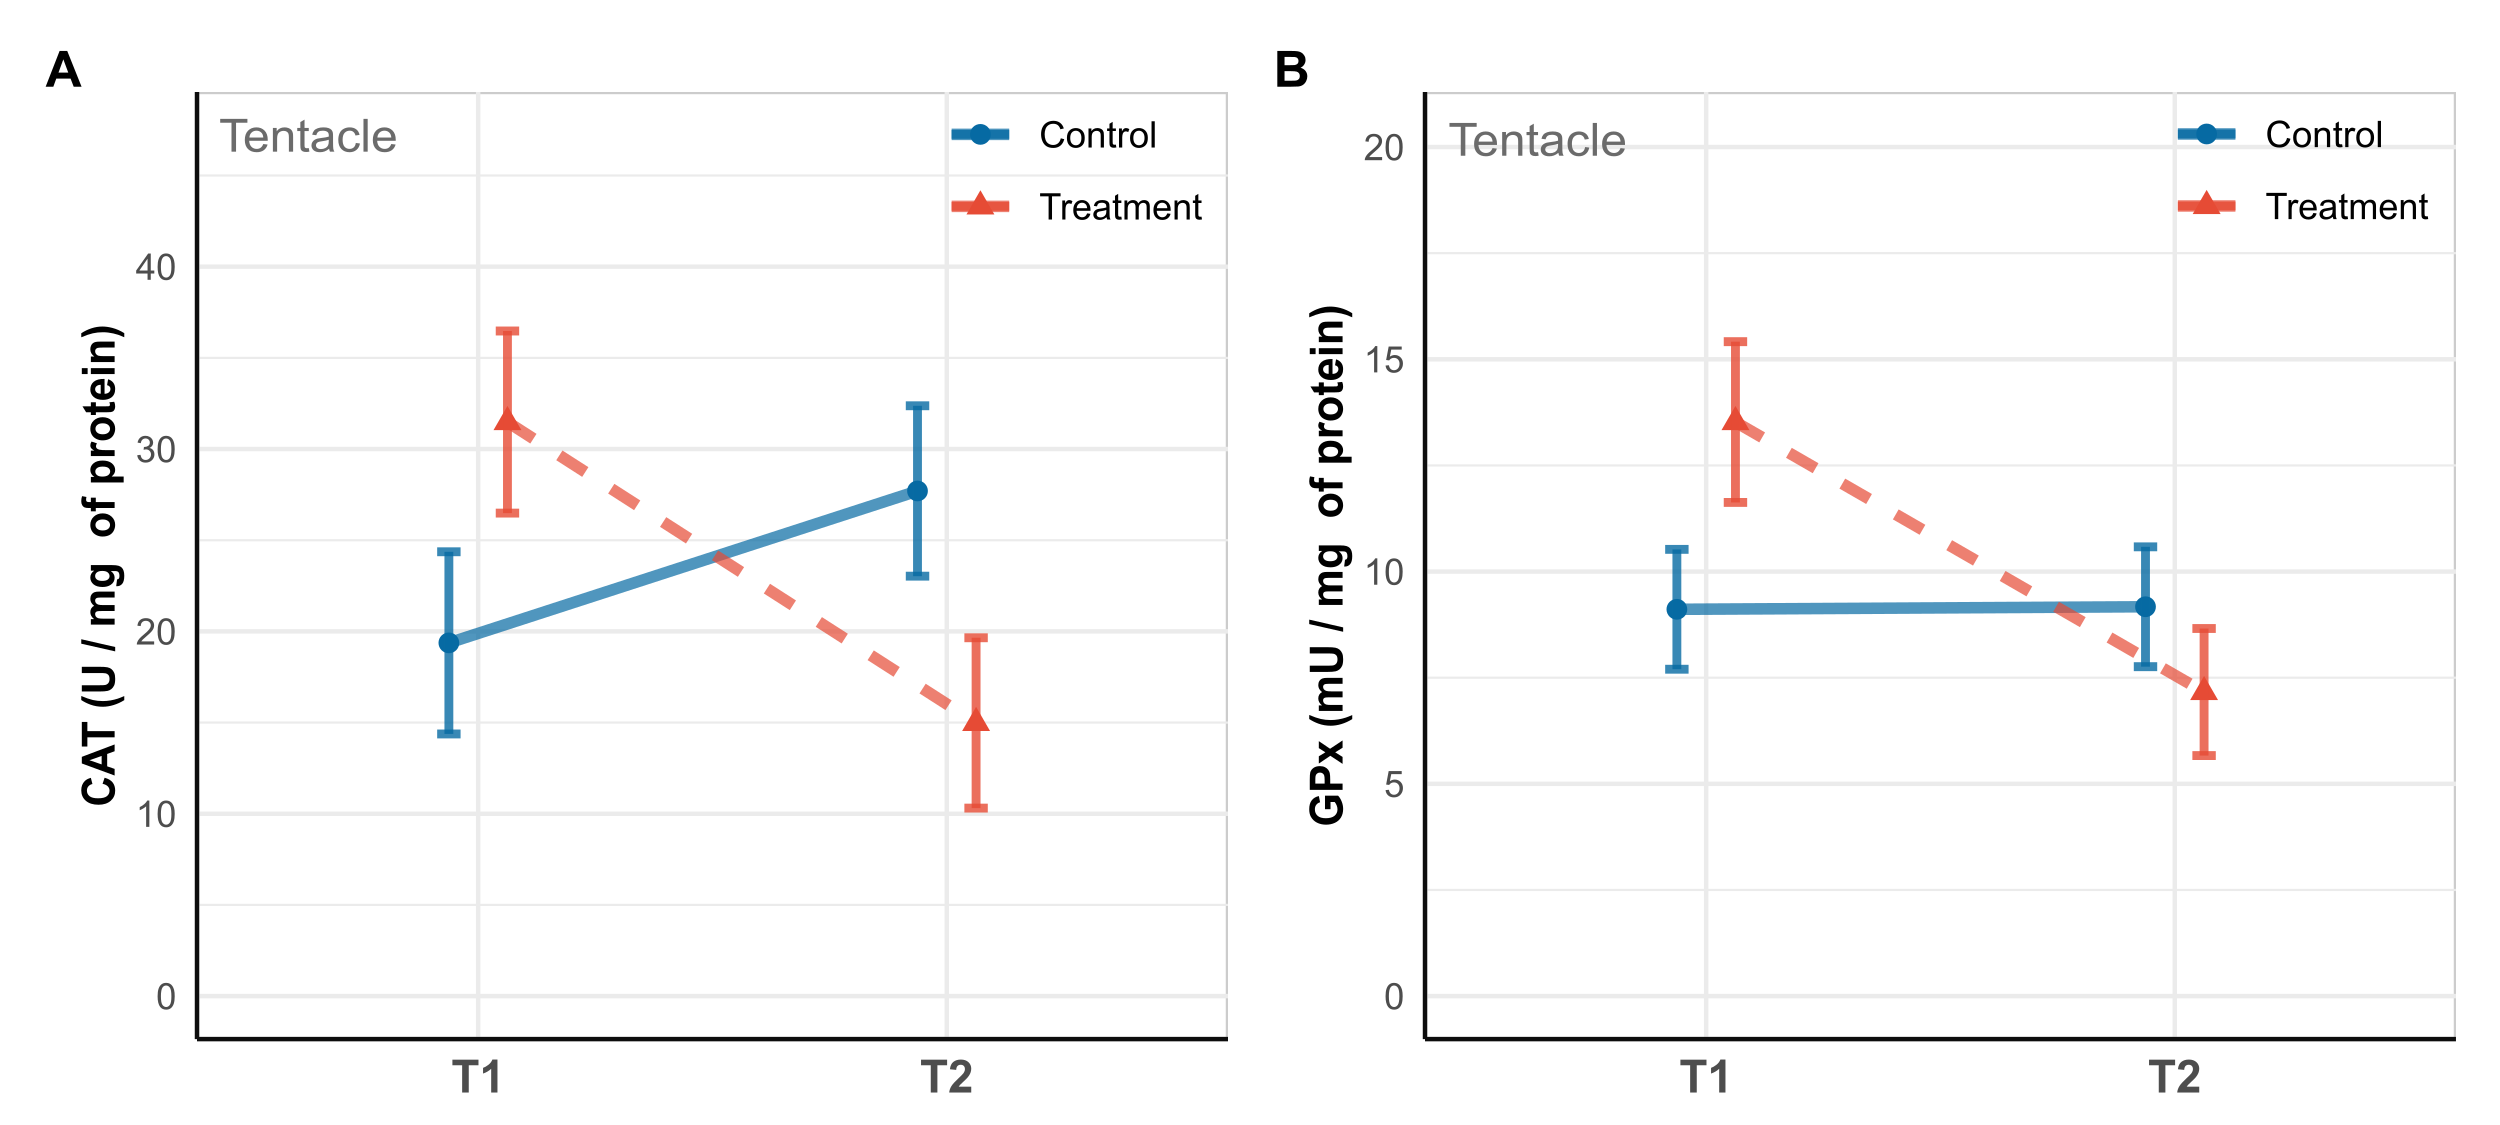
\includegraphics[width=0.8\textwidth]{Figura CAT_GPx.png}
    \caption{Model estimated marginal means with 95\% confidence intervals of control and bisected anemones, at T1 (4 weeks) and T2 (20 weeks), for variables that featured significant interaction effects: (A) tentacular catalase, (B) tentacular glutathione peroxidase.}
    \label{fig:emm1}  
\end{figure}

Neither columnar or tentacular total antioxidant capacity, measured as Trolox equivalent antioxidant capacity (TEAC; Figure \ref{fig:mda}.A) showed significant effects associated with treatment, time or their interaction. Columnar lipid peroxidation, measured as TBARS (Figure \ref{fig:mda}.B), showed no effect of treatment or interaction; although there was a non-significant trend towards lower lipid peroxidation at T2 ($F_{(1,32)}$= 6.63, p = 0.058). Tentacular lipid peroxidation was found to be lower on bisected individuals compared to control ones ($F_{(1,32)}$= 9.46, p = 0.025), but was not affected by time or interaction.

\subsection{Immune status parameters}
\label{subsec8}

No differences were detected on columnar or tentacular ACP (Figure \ref{fig:immune}.A) due to treatment, time or their interaction. Columnar ALP (Figure \ref{fig:immune}.B) was not significantly affected by time or interaction, but it featured a non-significant trend towards higher values in bisected anemones ($F_{(1,32)}$= 5.54, p = 0.088). There was no effect of treatment, time or interaction on tentacular ALP.

Regarding MPO activity (Figure \ref{fig:immune}.C), there was a significant effect of treatment ($F_{(1,32)}$= 14.37, p = 0.006) and treatment by time interaction ($F_{(1,32)}$= 15.05, p = 0.006) on columnar MPO, but no effect of time. Visual inspection of the estimated marginal means (Figure \ref{fig:emm3}) showed that control anemones had higher MPO activity at T1 than the rest of the experimental groups. Tentacular MPO activity was not affected by either variable or their interaction.

\begin{figure}[hbtp]
    \centering
    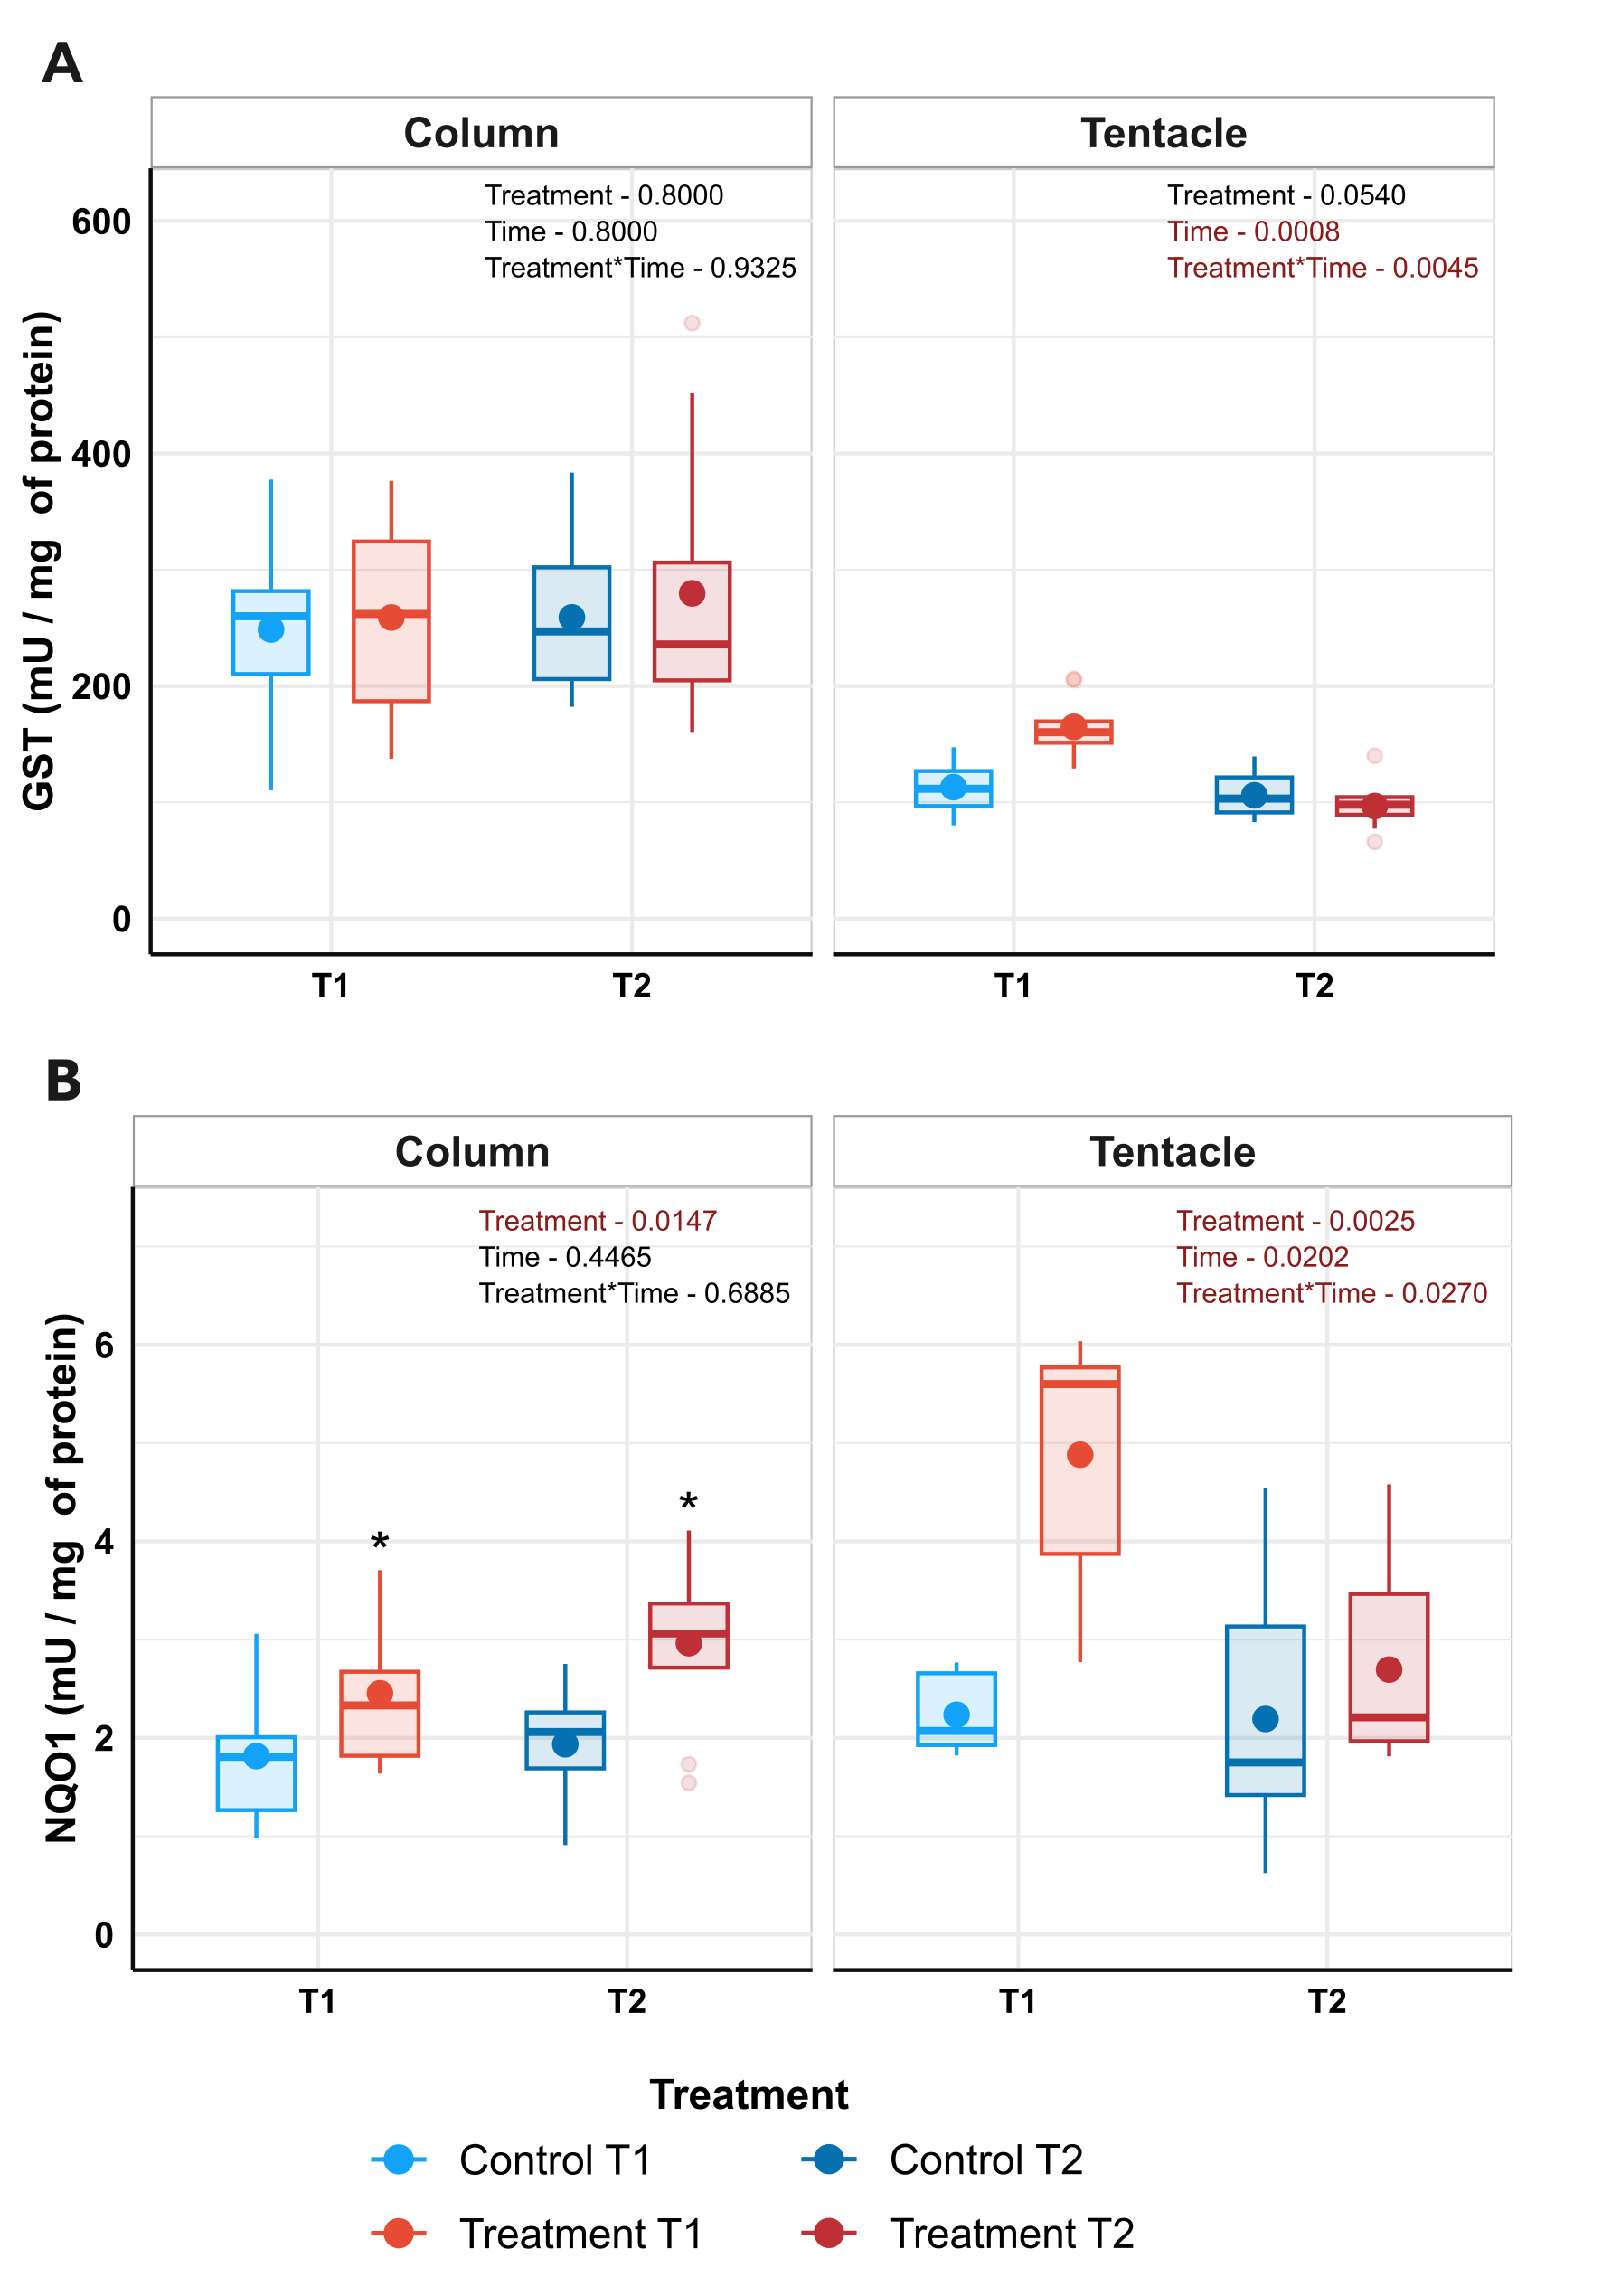
\includegraphics[width=0.6\textwidth]{fig_boxplot2.png}
    \caption{(A) Glutathione-S-transferase (GST) activity and (B) NAD(P)H quinone oxidoreductase 1 (NQO1) activity on column and tentacles of control and bisected anemones, at T1 and T2. Coloured dots represent the mean value. n = 9 per experimental group. Two-way ANOVA table is displayed on each panel, with p-values < 0.05 in red. Asterisks indicate significant differences due to treatment main effect. Effects of time not indicated.}
    \label{fig:gst}
\end{figure}

\begin{figure}[ht]
    \centering
    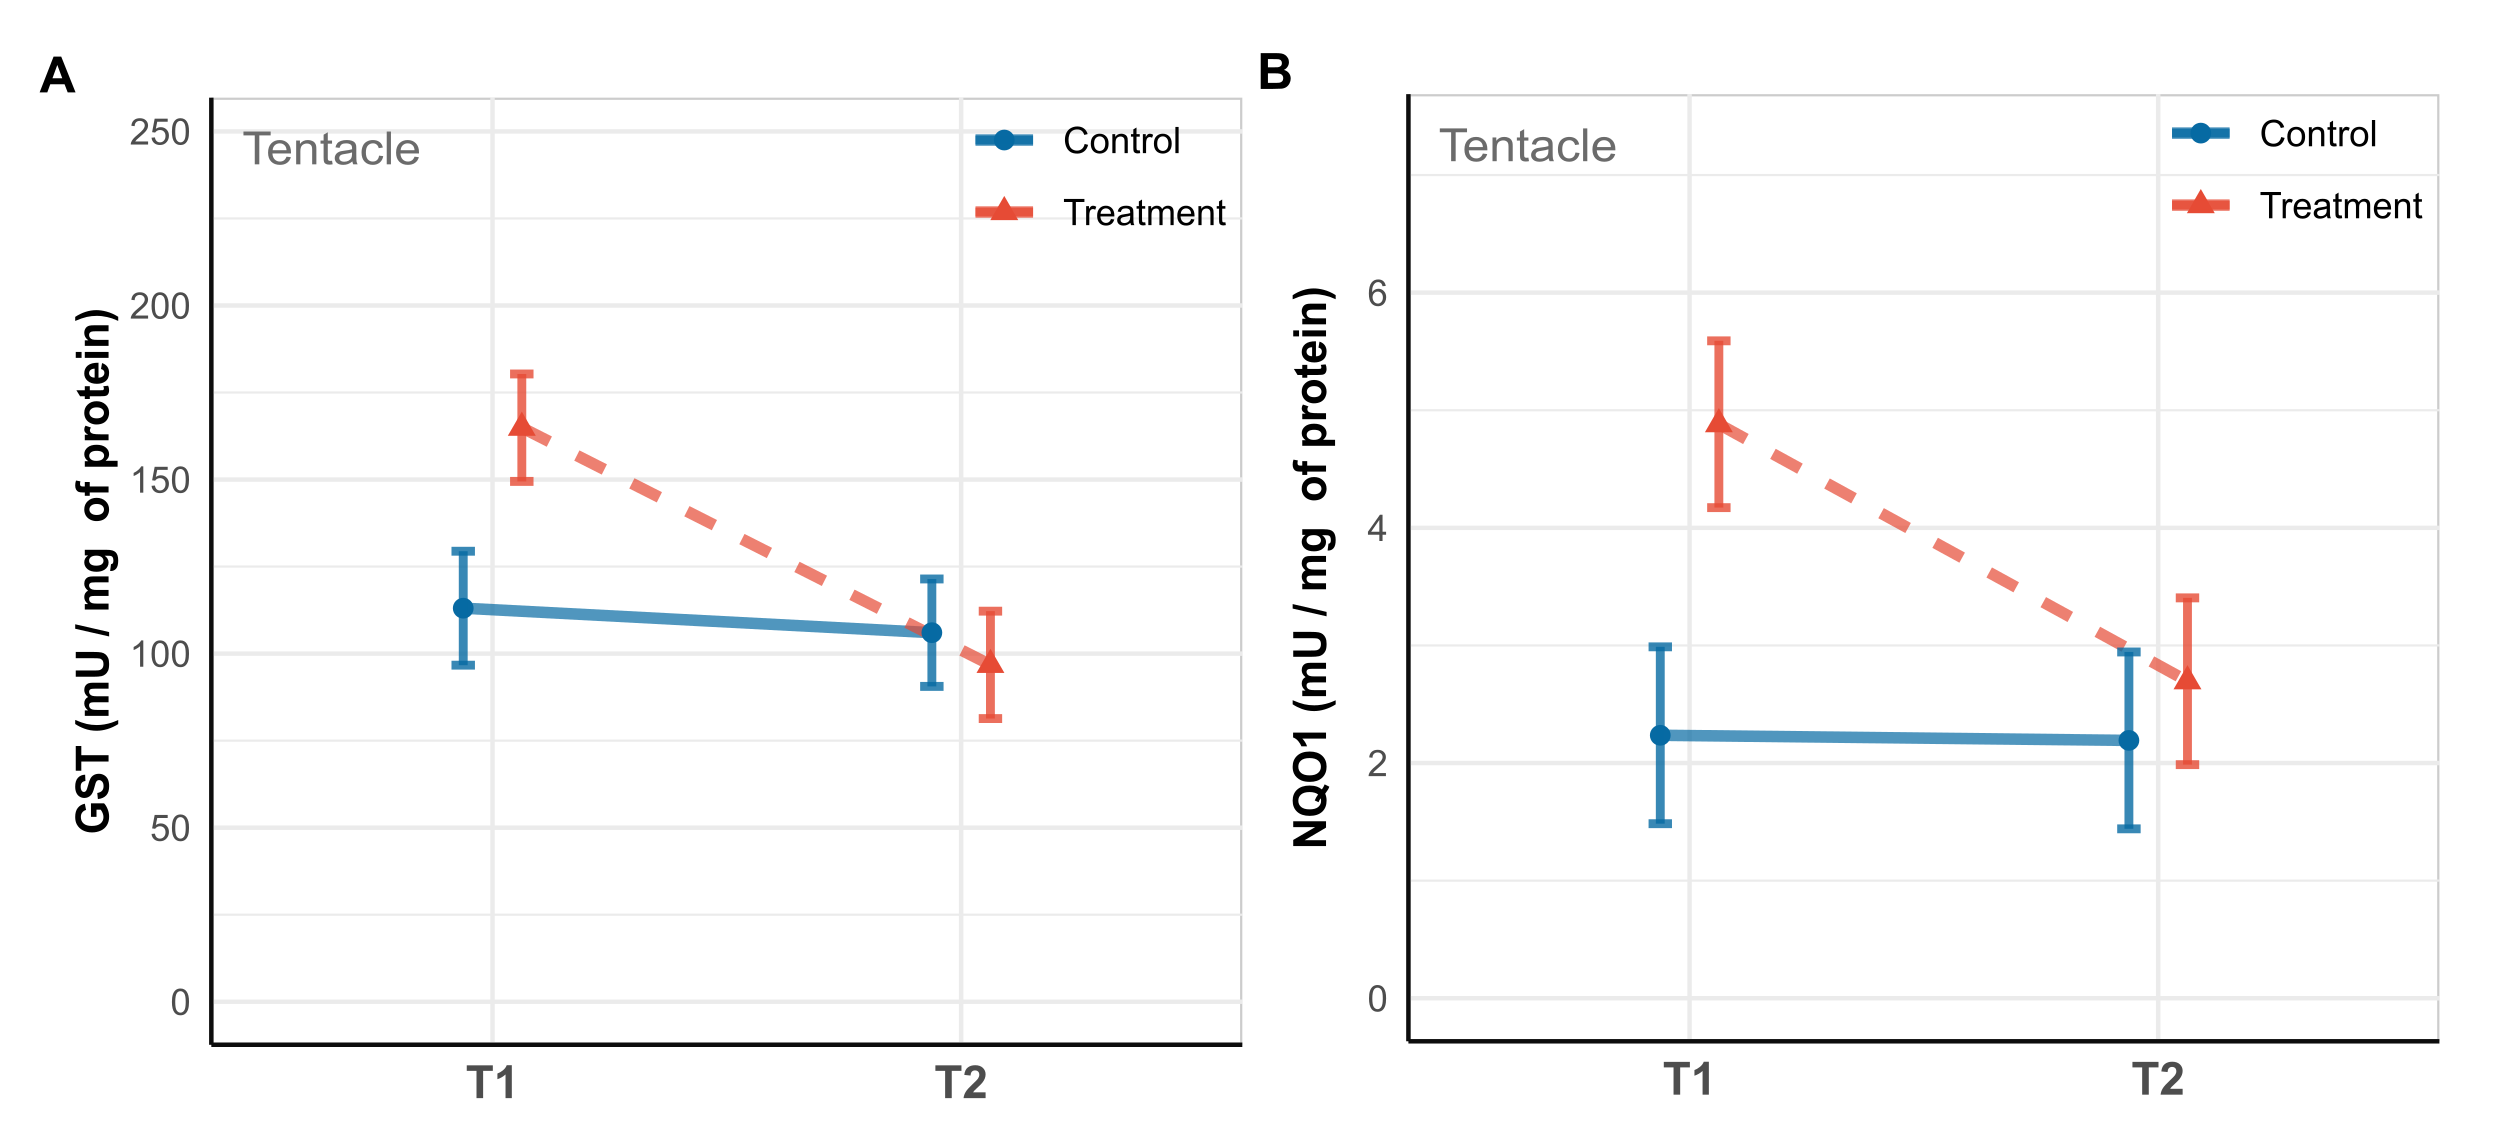
\includegraphics[width=0.8\textwidth]{Figura GST_DTD.png}
    \caption{Model estimated marginal means with 95\% confidence intervals of control and bisected anemones, at T1 (4 weeks) and T2 (20 weeks), for variables that featured significant interaction effects: (A) tentacular glutathione S-transferase, (B) tentacular NAD(P)H quinone oxidoreductase 1.}
    \label{fig:emm2}  
\end{figure}

\begin{figure}[hbtp]
    \centering
    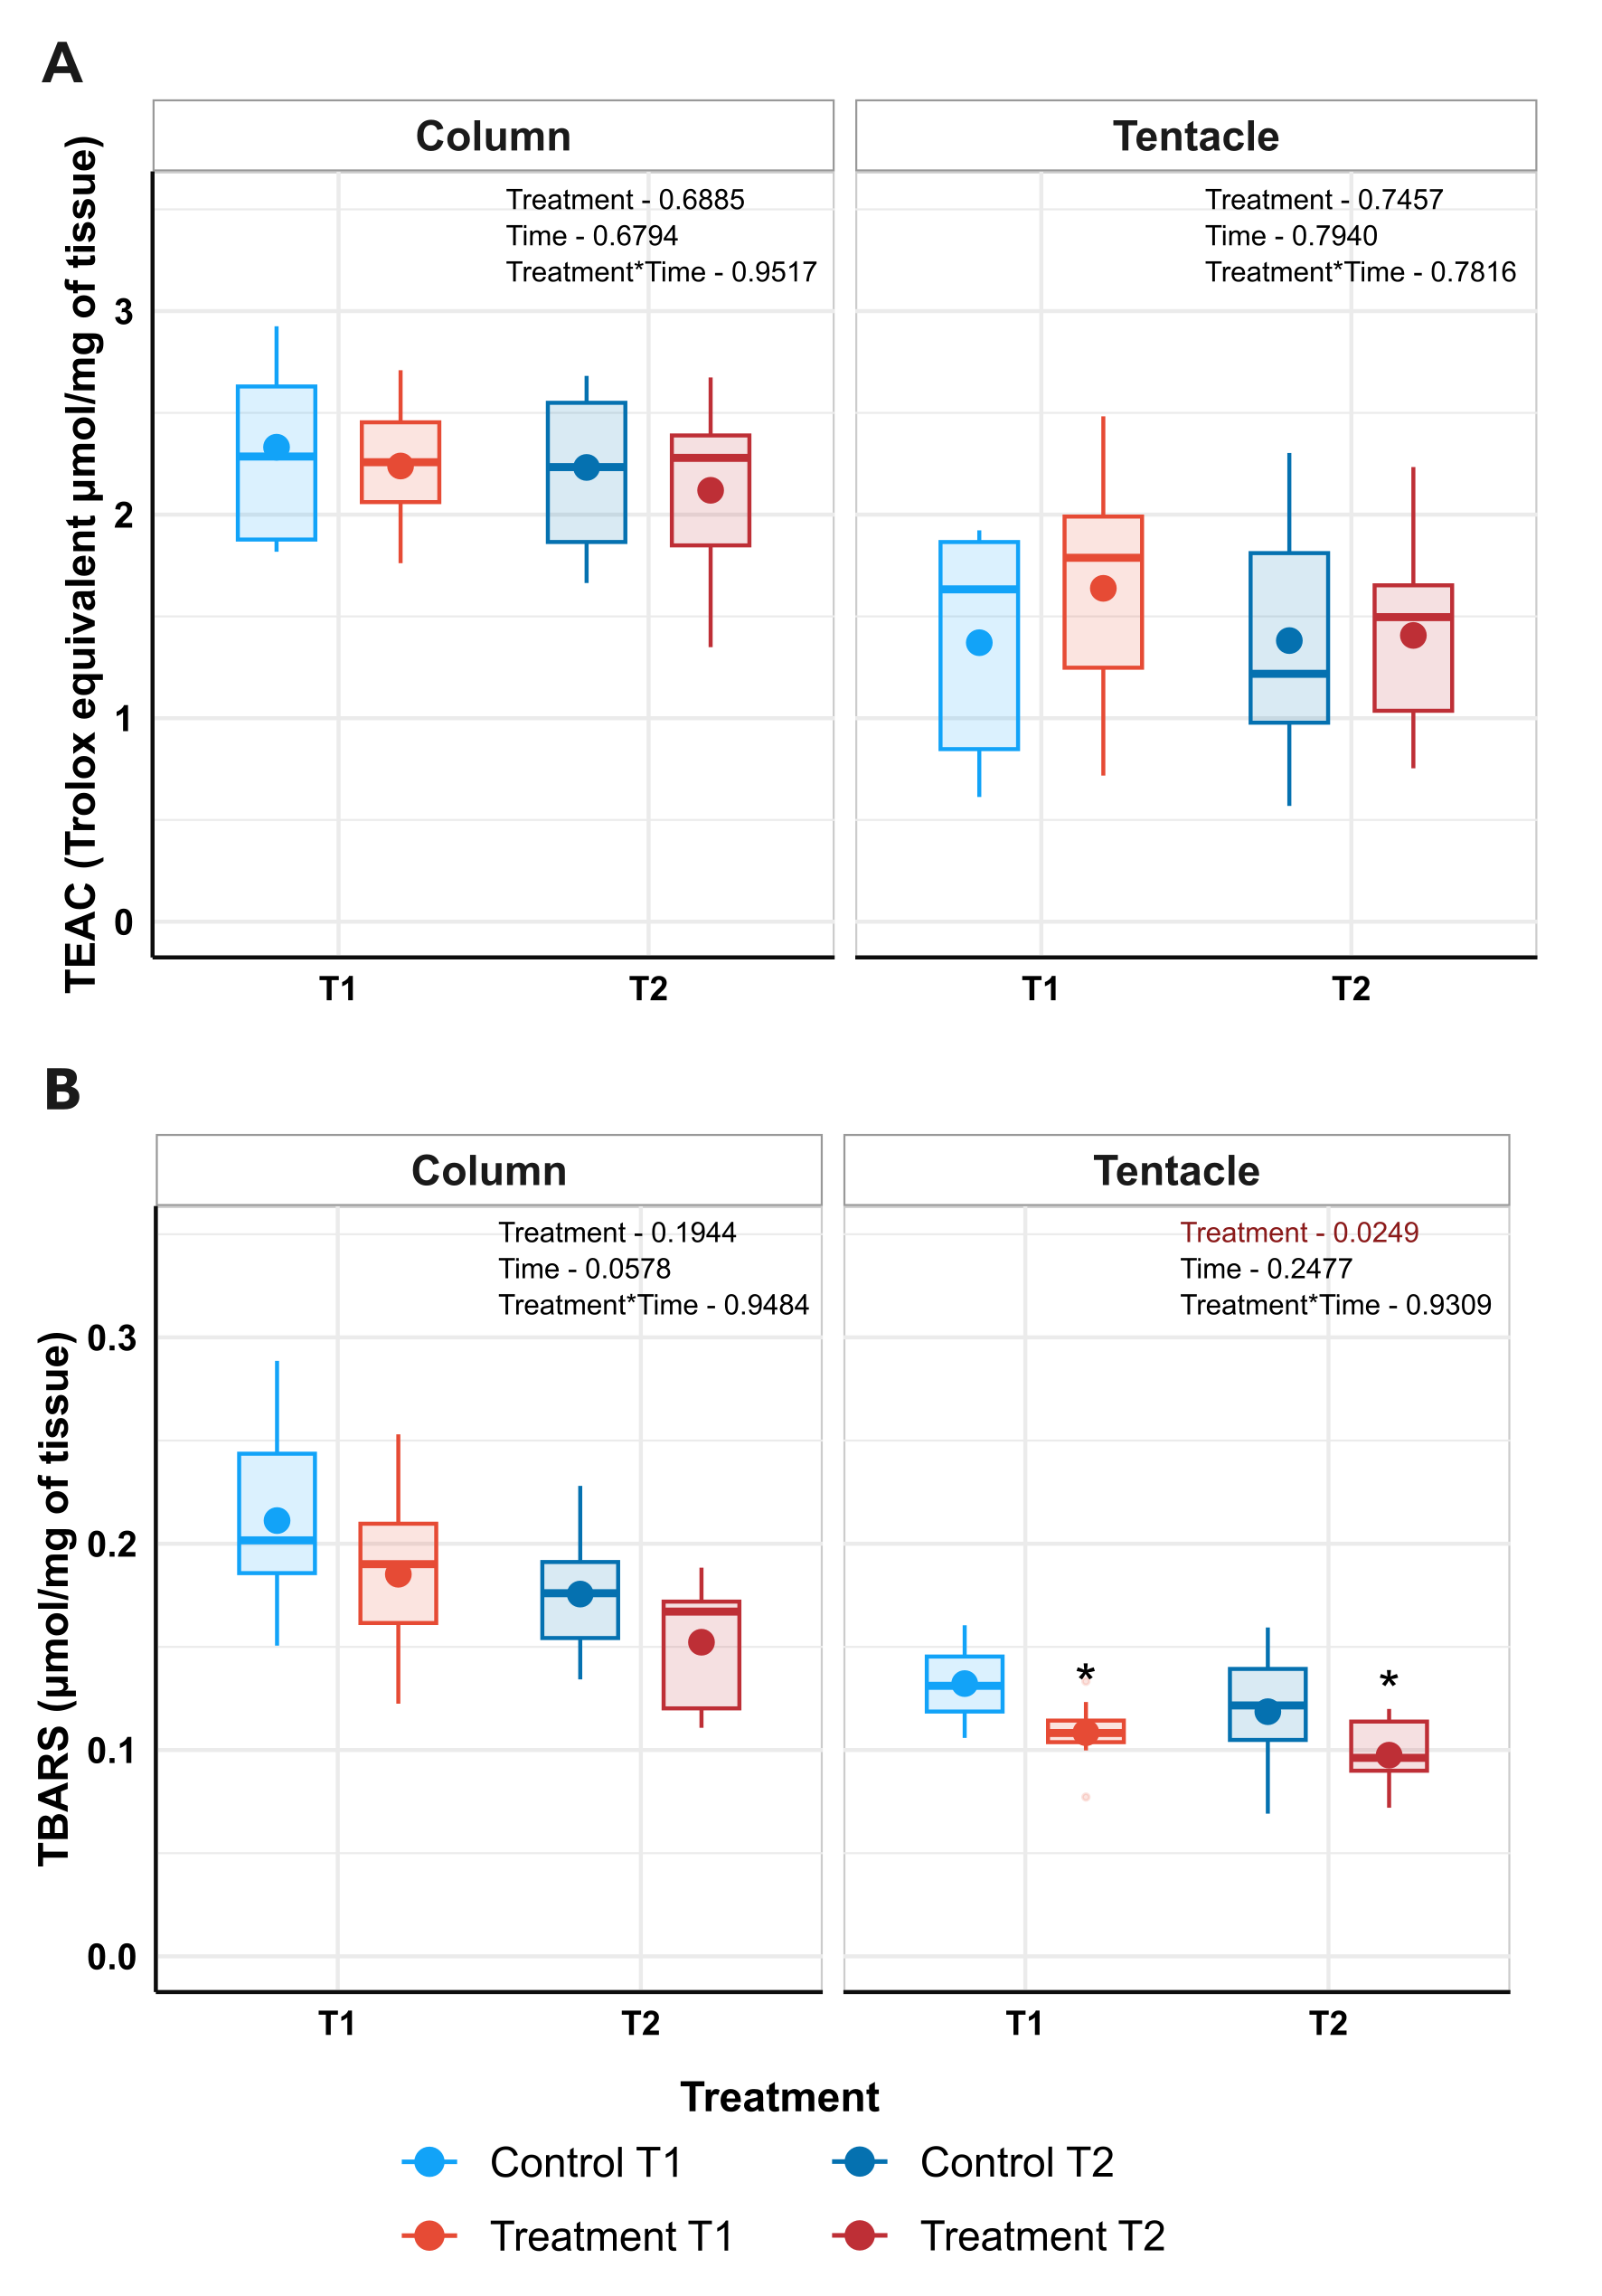
\includegraphics[width=0.6\textwidth]{fig_boxplot3.png}
    \caption{(A) Trolox-equivalent antioxidant capacity (TEAC) and (B) Malondialdehyde (MDA) concentration on column and tentacles of control and bisected anemones, at T1 and T2. Coloured dots represent the mean value. n = 9 per experimental group. Two-way ANOVA table is displayed on each panel, with p-values < 0.05 in red. Asterisks indicate significant differences due to treatment main effect. Effects of time not indicated.}
    \label{fig:mda}
\end{figure}

\begin{figure}[hbt]
    \centering
    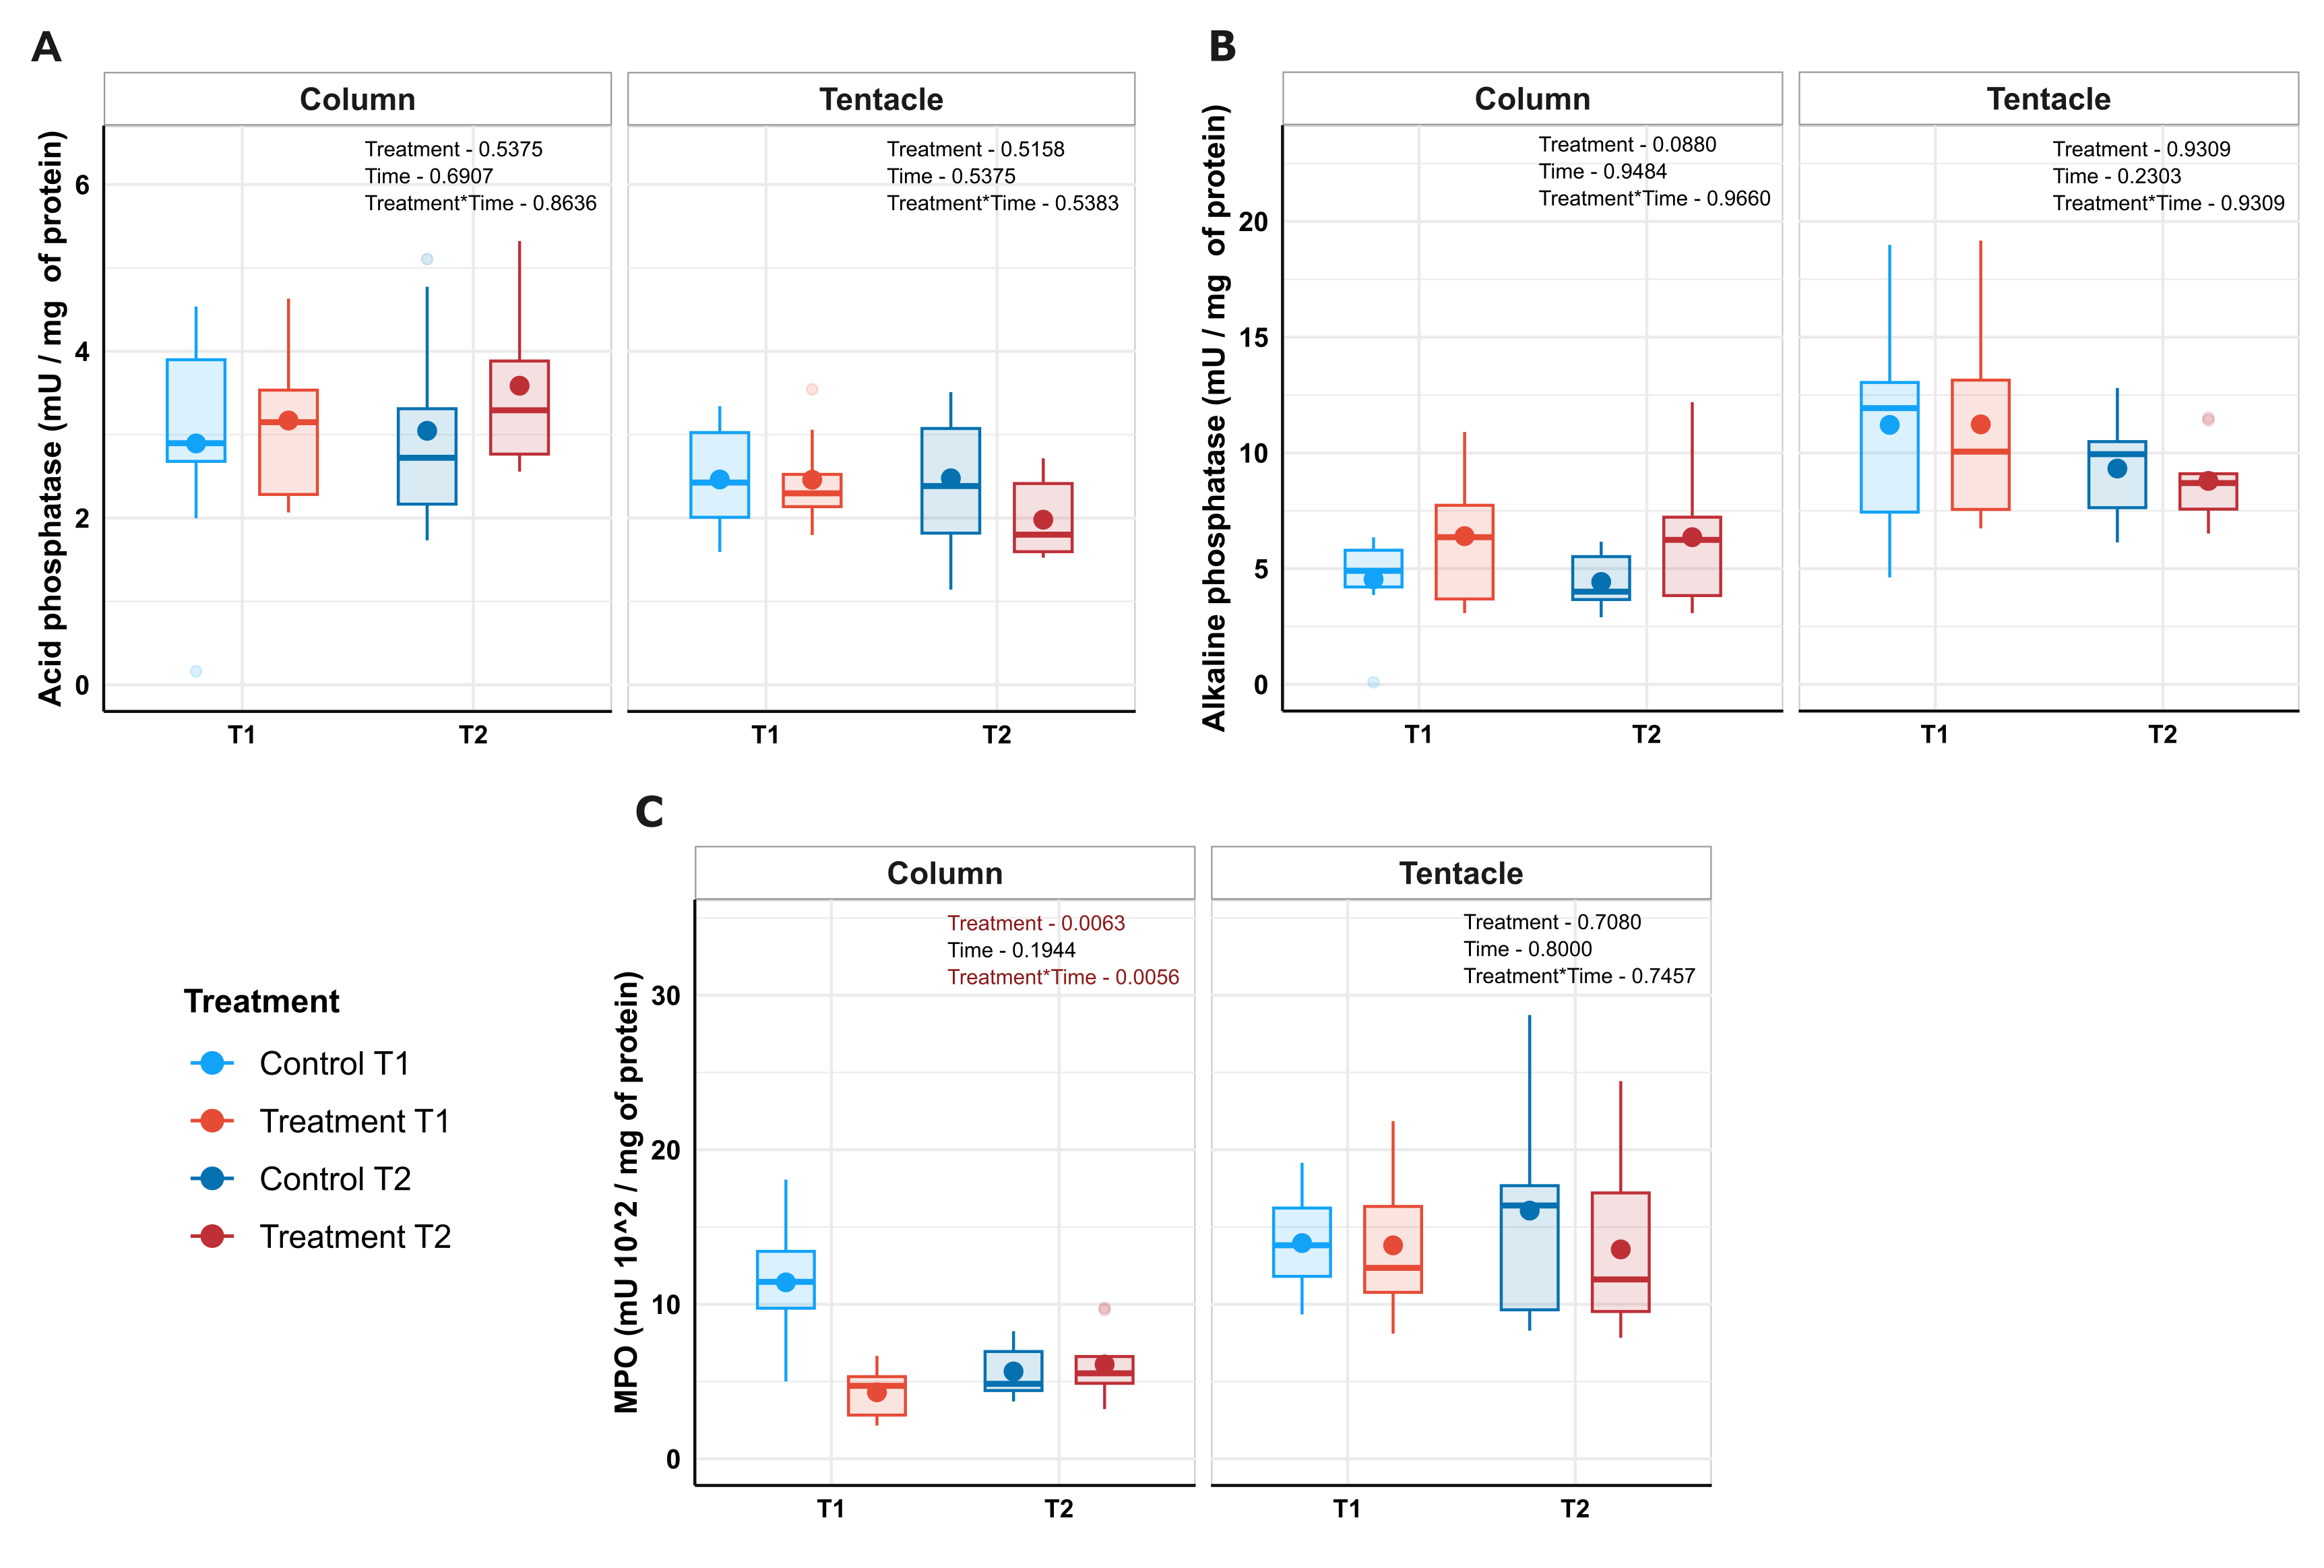
\includegraphics[width=1\textwidth]{fig_boxplot4.png}
    \caption{(A) Acid phosphatase (ACP), (B) alkaline phosphatase (ALP) and (C) myeloperoxidase (MPO) activity on column and tentacles of control and bisected anemones, at T1 and T2. Coloured dots represent the mean activity. n = 9 per experimental group. Two-way ANOVA table is displayed on each panel, with p-values < 0.05 in red. Asterisks indicate significant differences due to treatment main effect. Effects of time not indicated.}
    \label{fig:immune}
\end{figure}

\begin{figure}[ht]
    \centering
    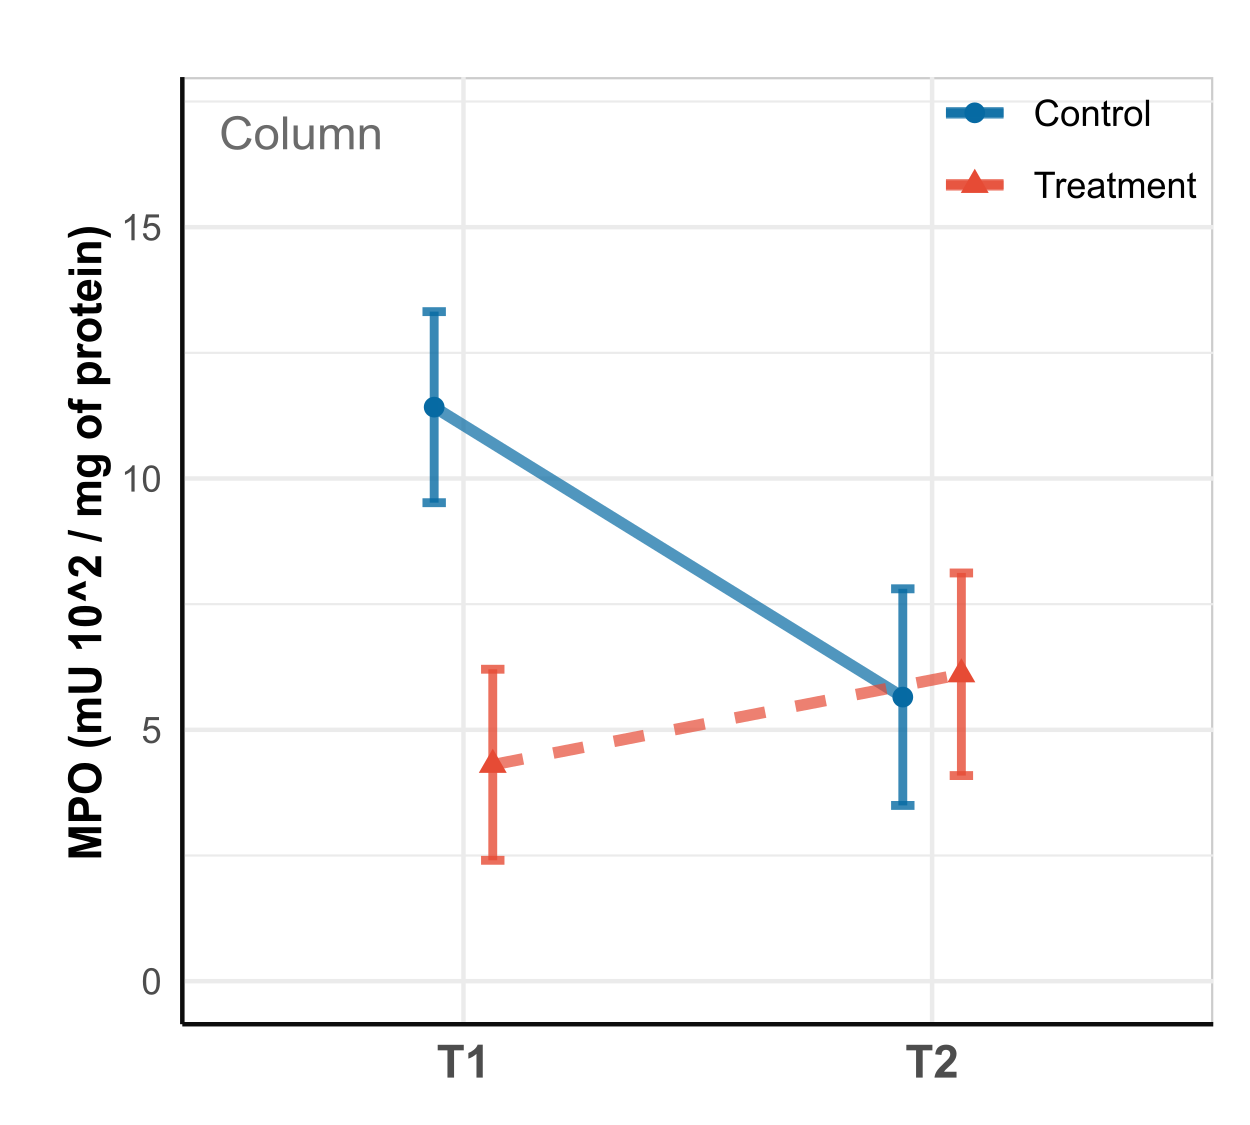
\includegraphics[width=0.4\textwidth]{Figura mpo.png}
    \caption{Model estimated marginal means with 95\% confidence intervals of control and bisected anemones, at T1 (4 weeks) and T2 (20 weeks), for columnar mieloperoxidase.}
    \label{fig:emm3}  
\end{figure}

\subsection{Principal Component Analysis}
\label{subsec9}

Permutation tests for $\psi$ and $\phi$ statistics were significant in both columnar variables and tentacular variables, indicating the presence of non-random correlations within the data and adequacy of PCA. In Figure \ref{fig:pca}, observations are grouped according to time point and treatment, and 95\% confidence ellipses were constructed, highlighting separation between experimental groups. Variables were overlaid as vectors.

For columnar variables, two principal components (PCs) were significant, and together they accounted for 51.4\% of the original data variance. PC1 represented 33.1\% (Confidence Interval (CI-95\%: 26.3-45.2) of this variation, and variables SOD, CAT, GPx, GST and MDA contributed significantly to it. PC2 explained 18.8\% (CI-95\%: 16.1-24.8), and MPO was the main contributor to this component. A slight separation can be observed between control observations, that tended to score positively for PC2, and bisected observations, that mostly scored negatively for this principal component.

Regarding tentacular variables, only PC1 was significant according to permutation tests, and it accounted for 35\% (CI-95\%: 28.4-47.5) of original data variance. CAT, GR, GST, ACP, ALP and MPO contributed more than expected by chance to this component. In this case, Treatment-T1 samples were separated from other groups, including bisected samples at T2 which overlapped with control observations. 

\begin{figure}[htp]
    \centering
    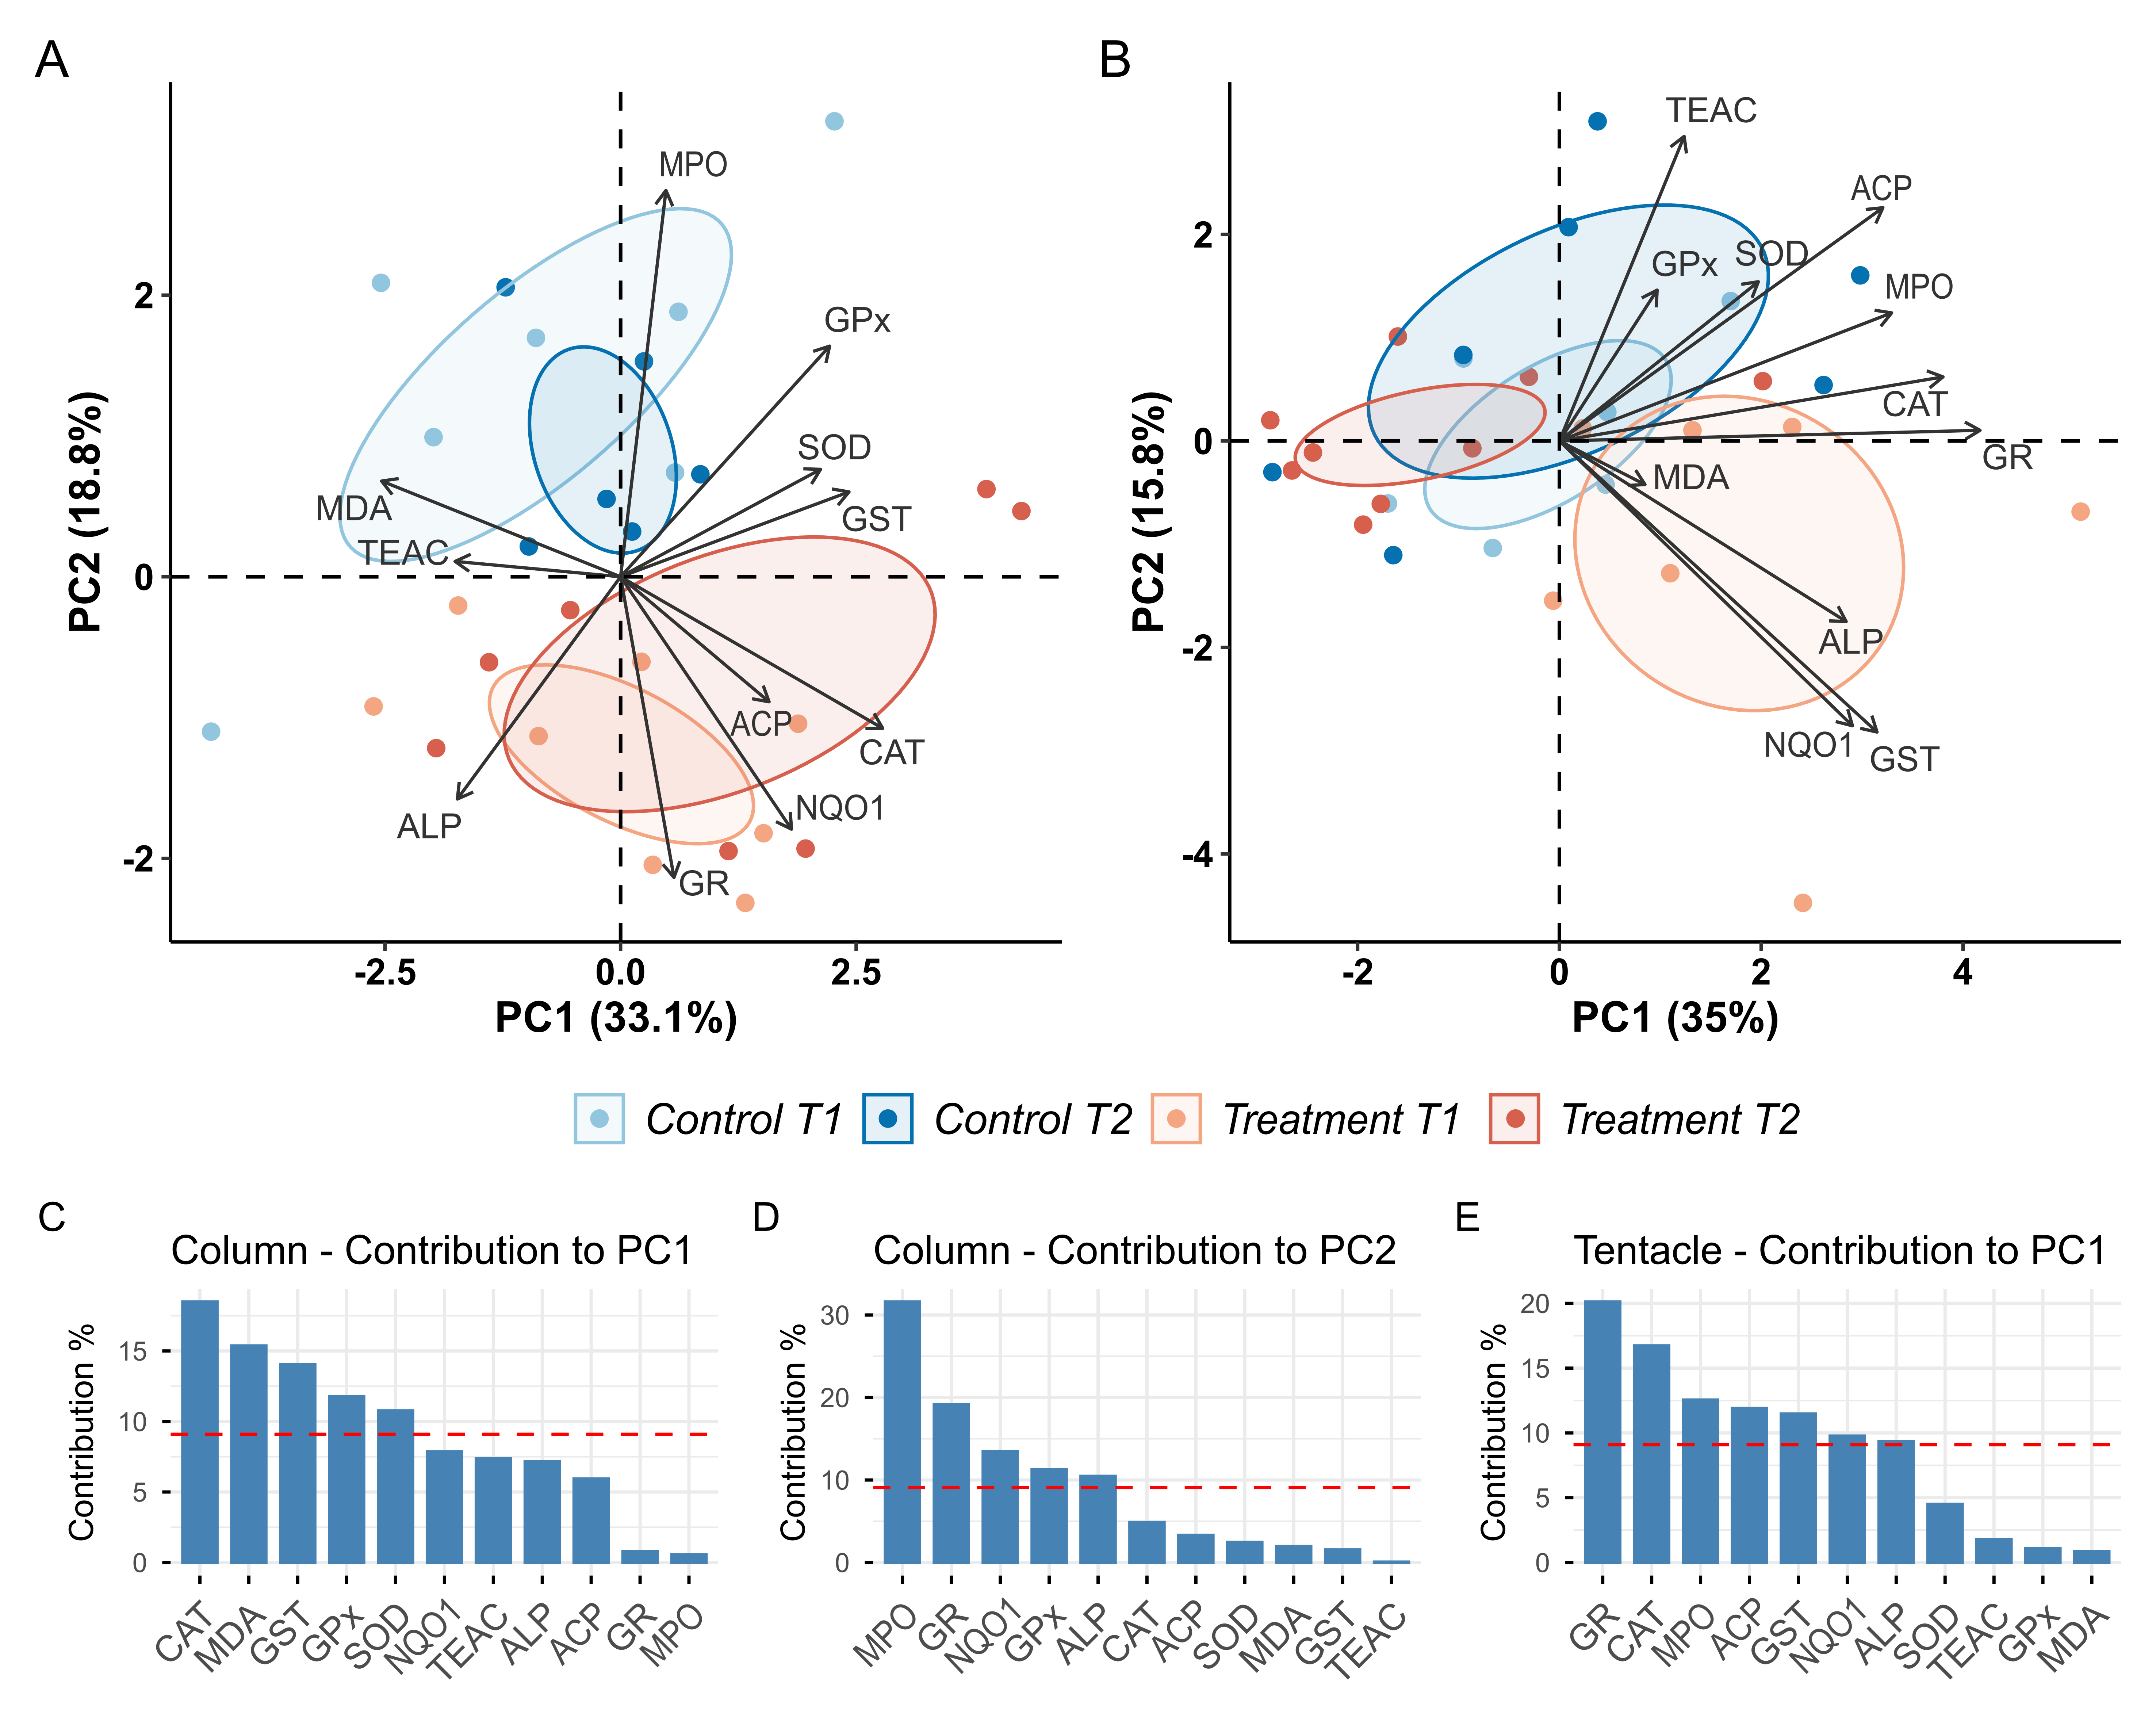
\includegraphics[width=1\textwidth]{fig_pca.png}
    \caption{(A) Biplot of PC1 and PC2 for columnar variables. Samples are grouped according to treatment, with 95\% confidence ellipses. (B) Biplot of PC1 and PC2 for tentacular variables. Samples are grouped according to treatment, with 95\% confidence ellipses. (C) Percentage contribution of columnar variables to PC1. (D) Percentage contribution of columnar variables to PC2. (E) Percentage contribution of tentacular variables to PC1. Red dashed lines indicate threshold of expected average contribution. SOD: superoxide dismutase; CAT: catalase; GPx: glutathione peroxidase; GR: glutathione reductase; GST: glutathione-S-transferase; NQO1: NAD(P)H quinone oxidoreductase 1; TEAC: trolox-equivalent antioxidant capacity; MDA: malondialdehyde; ACP: acid phosphatase; ALP: alkaline phosphatase; MPO; myeloperoxidase.}
    \label{fig:pca}
\end{figure}

\subsection{Histology}
\label{subsec10}

Observed histological sections displayed the typical three-layer organization found in cnidarians, consisting of an external epidermal tissue layer, an intermediate extracellular matrix layer called mesoglea, stained by Light Green SF due to presence of collagen fibers; and an internal gastrodermal tissue layer that hosts symbiotic zooxanthellae. This basic pattern was repeated throughout the body wall of the organism, but some modifications of the different layers appeared, such as mesenteries that emerge from the gastrodermis inside of the gastrointestinal cavity.

The wound area and surrounding mesoglea were located and monitored in sea anemones at the time of bisection, at 6 hours, at 24 hours and at 7 days after the procedure (Figure \ref{fig:hist1} \& \ref{fig:hist2}). At 0 hours, the wound area was open, and all three layers of the body wall were completely disrupted. Mesenteric filaments and waste material were found outside the gastrovascular cavity (Figure \ref{fig:hist1}.A). At 6 hours, the exposed mesoglea around the wound area was partially covered by cellular debris and components of the extracellular matrix. (Figure \ref{fig:hist1}.B). Some samples also featured aggregation of amoebocytes in the mesoglea (Figure \ref{fig:hist2}.B).

At 24 hours, mesoglea near the injury areas appeared lax and acquired a reticular or fibrillar appearance (Figure \ref{fig:hist2}.C). Amoebocyte presence was detected as well. Furthermore, all samples exhibited intrusion of extracellular matrix components into the epidermis and gastrodermis of the injury area, as evidenced by Light Green SF staining (Figure \ref{fig:hist3}). Seven days after the injury, macroscopic observation of the specimens revealed that the wound was closed, and some of them had already regenerated part of their column. Microscopic examination revealed a new body wall, characterized by thin epidermal and gastrodermal layers and separated by a very narrow mesoglea (Figure \ref{fig:hist1}.D). This new body wall ran parallel to pre-existing mesenteries, and some of the nearer mesenteries were connecting to the regenerated wall. Heavy amoebocyte recruitment was observed along the mesoglea of the new tissue (Figure \ref{fig:hist2}.D).

\begin{figure}[hbt]
    \centering
    \includegraphics[width=1\textwidth]{fig_histology1.png}
    \caption{Longitudinal section of the column of \textit{A. viridis} immediately after the injury (A), 6 hours post-injury (B), 24 hours post-injury (C) and 7 days post-injury (D). 5 µm sections stained with Masson-Golder thrichrome, highlighting collagen fibers and mesoglea in green. Yellow dashed line and arrow indicates bisection plane. Ep: Epidermis; M: Mesoglea; Gs: Gastrodermis, ms: mesenteries. Scale bars—(A) 100 µm; (B-C) 50 µm; (D) 250 µm.}
    \label{fig:hist1}
\end{figure}

\section{Discussion}
\label{sec4}

The possibility of reproducing the snakelocks anemone (\textit{Anemonia viridis}) in captivity via induction of their regeneration could be a major step towards conservation of this species in the Mediterranean Sea. The aim of this study was to explore the impact of inducing asexual reproduction of \textit{A. viridis} on the stress response associated with wound healing and regeneration of the missing body parts. Our results suggest that longitudinal bisection of the anemones is an effective methodology for this purpose, as it resulted in a high survival and prompted fast wound healing.

Oxidative status is a complex interplay of ROS generation and ROS scavenging by antioxidant defenses \citep{Gauron2013, Beaulieu2014}. The present study detected increases in columnar and tentacular antioxidant enzyme activities in regenerating anemones at one or both time points (4 weeks and 20 weeks after the injury). The affected enzymes were mainly glutathione-dependent enzymes (such as GPx, GR and GST) and/or $\mathrm{H_2O_2}$-processing enzymes (CAT and GPx). Glutathione has a central position in antioxidant metabolism, and it has been shown to intervene in regenerative processes in invertebrates \citep{Bijnens2021}. Available reduced glutathione can be used by GPx for $\mathrm{H_2O_2}$ reduction, can be conjugated with exogenous xenobiotics by GST, or can scavenge pro-oxidative molecules directly \citep{Couto2016}. GR, a key enzyme in the recycling of reduced glutathione, showed higher activity in bisected anemones regardless of temporal sampling point, which could be linked to an increased usage and turnover of this antioxidant. NQO1, on the other hand, catalyzes the reduction of quinones, bypassing formation of semiquinones and the subsequent ROS production \citep{Atia2020, Ross2021}. The increased activity of this enzyme on bisected anemones could be the consequence of a greater generation of endogenous quinones, as these have been found to induce NQO1 expression in mammalians \citep{Atia2020}. NQO1 also has superoxide scavenging activity, and has been reported to be over-expressed in mammalian tissues where SOD expression is low \citep{Dinkova-Kostova2004, Siegel2004}. Ultimately, a higher NQO1 activity could offer an extra layer of antioxidant protection against the oxidative stress associated with the metabolic activation known to occur during regeneration processes \citep{Atia2020, Mack2025}. The lack of changes in Trolox-equivalent antioxidant capacity (TEAC) suggests that, within the studied time range, non-enzymatic antioxidants (such as thiol groups, uric acid, and vitamins C and E) are not the main pathway to scavenge ROS. However, \citet{LaCorte2025} reported a peak in total oxyradical scavenging capacity at 24 hours after tentacle amputation in \textit{A. viridis}, which supports the idea that low molecular weight antioxidants play an important role in the early wound healing response, but might be replaced by enzymatic antioxidants during and after the subsequent regeneration process. 

\begin{figure}[bht]
    \centering
    \includegraphics[width=1\textwidth]{fig_histology2.png}
    \caption{Mesoglea near the wound area of \textit{A. viridis} immediately after the injury (A), 6 hours post-injury (B), 24 hours post-injury (C) and 7 days post-injury (D). 5 µm sections stained with Masson-Golder thrichrome, highlighting collagen fibers and mesoglea in green. Ep: Epidermis; M: Mesoglea; Gs: Gastrodermis, ms: mesenteries; mu: muscle fibers; arrowheads: zooxanthellae. Scale bars — 25 µm.}
    \label{fig:hist2}
\end{figure}

Columnar lipid peroxidation was found to be similar for all experimental groups based on the TBARS assay, and tentacles of regenerating anemones featured significantly lower lipid peroxidation than control samples. This lack of oxidative damage despite the detected increase in the antioxidant parameters suggests a scenario in which, despite some level of ROS production, antioxidant mobilization was able to prevent oxidative damage to cellular lipids and maintain homeostasis. This would mean that the sea anemones were able to protect themselves from the pro-oxidative conditions they faced during regeneration. Previous works report the robustness of this species and other symbiotic anthozoans to oxidative damage caused by environmental stress \citep{Coll2025}. This is likely linked to the evolution of symbiosis and the wide variations in oxygen partial pressure that take place between daytime and nighttime due to zooxanthellae photosynthesis \citep{ Richier2005, Casado-Ameza2016}. Adaptations to symbiosis in this and other anthozoan species have been studied extensively, and include a more robust antioxidant system than found in non-symbiotic sea anemones \citep{Richier2003, Richier2005, Casado-Ameza2016, Pey2017, Cotinat2022}. 

PCA results for columnar data also support this scenario, since several antioxidant enzymes and MDA levels contributed significantly to PC1 in opposite senses, indicating negative correlation between these parameters (Figure \ref{fig:pca}). PC1 could thus be interpreted as a metric of redox state, which was responsible for about 33\% of the dataset variance. Notably, enzymes contributing significantly to this component were limited to CAT, GST, GPx and SOD; despite the fact that columnar activity for most of these enzymes was not affected by treatment in univariate analysis. However, despite PC1 explaining a third of the original variance, only PC2 was able to clearly separate control and bisected observations. This suggests that redox state, based on the aforementioned enzymes and TBARS, was not the main driver of multivariable differences between control and bisected anemones. Contributing variables to PC2, such as MPO and GR (and to a lesser extent GPx), might be more relevant in shaping the physiological state of bisected anemones.

The antioxidant response of the column was generally found to be sustained over our two temporal sampling points, but enzymes that increased their activity in tentacular extracts all experienced a decline at T2, sometimes returning to levels similar to or under the control group (Figures \ref{fig:emm1}\&\ref{fig:emm2}). PCA for tentacular samples also highlighted this tendency at the multivariate level (Figure \ref{fig:pca}). The different degree of complexity and organization of the cnidarian body wall between tentacles and column might be the cause. Even though they are both composed of the same three layers, the tentacle body wall is thinner and lacks some of the more complex gastrodermal and epidermal specializations featured on the column, such as mesenteries, acrorhagi, or parietal and retractor muscles \citep{Harrison1991, Jahnel2014}. Moreover, previous studies on tentacle regeneration show that wound healing after tentacle amputation occurs within 24 hours in \textit{A. viridis} \citep{Parisi2021, LaCorte2023}, while our histological observations show that the column wound was not fully closed until 7 days post-injury.

Alkaline phosphatases (ALP) are one of the first enzymes to act in inflammatory processes, and high expression levels of this enzyme have also been reported during regenerative processes in \textit{A. viridis} \citep{Abe2001, Mauro2021, Parisi2021}. Lysosome hydrolases (such as acid phosphatase) (ACP) are considered regeneration markers in invertebrates, and both acid and alkaline phosphatases have been linked to epithelial cell and nematocyst differentiation in \textit{Hydra} \citep{Lentz1962, Orlando1991, Trapani2016, Konada2020}. In contrast with the evident antioxidant response, we detected no differences in ACP and ALP activity between control or bisected anemones throughout the study. \citet{Parisi2021} reported increases to ALP activity in \textit{A. viridis} after tentacle amputation extending to 14 days post-injury. This discrepancy with our results suggests that the enzymatic inflammatory response occurring after an injury is not detectable after 4 weeks post-injury. Histological examination supports this idea, as it confirmed that wound healing occurred within the first week after the injury in the case of longitudinal bisection (Figure \ref{fig:hist1}).

We registered higher columnar MPO activity in control anemones at T1 than in bisected anemones, but also higher than both groups at T2. Furthermore, PCA analysis highlighted MPO as the only significant contributing variable to PC2, which cleanly separated control and bisected anemones. MPO is a peroxidase typically associated to macrophages in vertebrates, as it is involved in the respiratory burst occurring during phagocytosis and phagosome digestion \citep{Klebanoff2005, Lin2024}. Phagocytic activity of amoebocytes has been described extensively in Hexacorallia, and ROS production has been detected after inducing amoebocytes with yeast and lipopolysaccharide extracts \citep{Hutton1996, Olano2000, Snyder2021, Fabrello2023}. Our results lead us to believe that, at 4-weeks post-injury, MPO  activity could be impaired to some degree in comparison to the high levels found in the control animals. The role of MPO in \textit{A. viridis} amoebocytes is thus likely more relevant during the early stages of wound-healing taking place in the first weeks post-injury, when the animal is more susceptible to infections due to the disruption in its body wall.

To complement biochemical assays, we performed a histological descriptive analysis of the wound healing process in snakelocks anemone during the first week after longitudinal bisection. Wound healing in anthozoans follows similar phases to those described in bilateral animals: (i) coagulation or clot formation, (ii) recruitment of immune cells, (iii) proliferation and re-epithelisation, and (iv) tissue remodeling \citep{Palmer2011, Parisi2021, LaCorte2023}. Our results from histological monitoring of \textit{A. viridis} specimens after suffering a complete longitudinal bisection match these four phases. We observed signs of clot formation at 6 h (Figure \ref{fig:hist1}), where the previously exposed mesoglea appeared partially covered in cellular debris that stained with acid fuchsin, as reported in previous findings by \citet{Palmer2011, LaCorte2023}. Some other authors report epithelial reorganization to seal exposed mesoglea after injuries in anthozoans \citep{Meszaros1999}, which also match some of the observations from this study, particularly 24 hours post-injury.

The heavy amoebocyte presence that was found in samples at 24h and 7d (Figure \ref{fig:hist2}) could be related to recruitment and/or proliferation of these cells during phases (ii) and (iii) of wound healing, due to their role in cnidarian immunity. Similarly to findings by \citet{Parisi2021}, we detected qualitative alterations in mesoglea organization at 6 h and 24 h post-injury, where the extracellular matrix became clearly organized in fibrils (Figure \ref{fig:hist2}). Light Green SF staining also revealed the presence of collagen in the epidermis and gastrodermis near the wound area, likely the result of infiltration of extracellular matrix components from the mesoglea (Figure \ref{fig:hist3}). In the same study, \citet{Parisi2021} detected evidence of collagen deposition during regeneration by mesoglea fibroblast-like cells, and proposed that these cells differentiate from hyaline amoebocytes. While the role of amoebocytes in collagen deposition has been a subject of debate \citep{Larkman1984}, our observations seem to broadly match these hypothesis. 

\begin{figure}[htb]
    \centering
    \includegraphics[width=0.6\textwidth]{fig_histology3.png}
    \caption{Detail of an area adjacent to the bisection plane at 0 h (A) and 24 h (B) post-injury. Green light infiltration (arrohead) from mesoglea (M) is observable in the epidermis (Ep) and gastrodermis (Gs) in an area adjacent to the injury at 24 hours. 5 µm sections stained with Masson-Golder thrichrome. Yellow dashed line and arrow indicates bisection plane. Scale bars — 100 µm.}
    \label{fig:hist3}  
\end{figure}

Although these results are promising for the application of this technique to reproduce anemones, there are still limitations that are to be considered during interpretation of results. As shown by histological observations, wound healing after longitudinal bisection of the column takes place within one week. The lack of measurements for biochemical parameters during this window of time limits our ability to link histological results with biochemical markers at later time points. Applying both approaches during this early stages of wound healing will improve understanding of regeneration processes in this species and similar organisms. While \textit{in vitro} enzymatic activity assays are accessible and simple methods of quantifying enzymatic antioxidants and immune enzymes, their \textit{in vivo} activity may be affected by differential cellular compartmentalization of enzyme isoforms or post-transcriptional modifications \citep{Noctor2016}. \textit{A. viridis} displays a remarkable diversity of first-phase antioxidant enzymes isoforms, distributed in different cell compartments between the animal host and the dinoflagellate symbiont \citep{Richier2003, Merle2007, Pey2017}. Hence, \textit{in vitro} enzymatic activity measurements would ideally need to be backed up with gene expression assays to better comprehend the role of antioxidant responses during regeneration. Similarly, despite the wide usage of TBARS assay due to its simplicity and inexpensiveness, several authors have raised concerns about its specificity \citep{Horak2010, AguilarDiaz2020}. Additionally, sample handling and storage variations can artificially inflate TBARS, which limits comparability of results between different laboratories \citep{AguilarDiaz2020}. While the assay is generally considered appropriate for intra-experimental comparisons between groups, the fact that TBARS was our only oxidative damage marker means different oxidative balance scenarios are not completely out of the question. These limitations could be mitigated in the future by using complementary oxidative damage assays in addition to TBARS.

Some gaps in knowledge arise from the results of the present study. A novel research question lies in the number of successive divisions a single anemone is able to withstand, as it will be a limiting factor for the application of this technique in the aquaculture industry. Another important aspect of regeneration is the range of environmental and physiological conditions in which it can take place (physiological niche for regeneration as introduced by \citet{Mack2025}). For example, external environmental parameters such as water temperature can impact invertebrates severely and interfere in wound healing and regeneration processes, increasing mortality \citep{LaCorte2025}. Our data was obtained from anemones during winter, but surface water temperature is highly variable during the year in Mediterranean regions. Hence, future research examining the intra-annual variation of the wound healing and regeneration response will valuably complement the present study

Finding reproduction techniques that are viable to implement in captivity and do not impair the animals physiology is vital to develop conservation measures for the snakelocks anemone. Our results show that vegetative asexual reproduction of this anemone can be induced artificially without detectable impairment on immune and oxidative balance of the animals up to 20 weeks after the injury. This methodology leads to a rapid increase of stock size, which can also reduce the current dependence on natural populations to supply individuals for human consumption. More importantly, it is a starting point to develop and achieve reliable sexual reproduction in captivity, a milestone that will be crucial to fully address the conservation issue this species currently faces in the Mediterranean Sea.


\section*{Acknowledgments}

This work was carried out thanks to funding from "ORTIMAR Project: Strategies for captive reproduction of the sea nettle (\textit{Anemona sulcata}) to optimize its reintroduction into the natural environment", framed in the Pleamar Program with the collaboration of the Biodiversity Foundation of the Ministry for the Ecological Transition and the Demographic Challenge and co-financed by the European Maritime and Fisheries Fund (FEMP). We also thank Ross W. Murphy for proof-reading and language revision.

\bibliographystyle{elsarticle-harv} 
\bibliography{Bibliography}


\end{document}

\endinput
%%
%% End of file `elsarticle-template-harv.tex'.